% CVPR 2025 Paper Template; see https://github.com/cvpr-org/author-kit

\documentclass[10pt,twocolumn,letterpaper]{article}

%%%%%%%%% PAPER TYPE  - PLEASE UPDATE FOR FINAL VERSION
\usepackage{cvpr}              % To produce the CAMERA-READY version
% \usepackage[review]{cvpr}      % To produce the REVIEW version
% \usepackage[pagenumbers]{cvpr} % To force page numbers, e.g. for an arXiv version
\usepackage[accsupp]{axessibility}  % Improves PDF readability for those with disabilities.

% Import additional packages in the preamble file, before hyperref
%
% --- inline annotations
%
\newcommand{\red}[1]{{\color{red}#1}}
\newcommand{\todo}[1]{{\color{red}#1}}
\newcommand{\TODO}[1]{\textbf{\color{red}[TODO: #1]}}
% --- disable by uncommenting  
% \renewcommand{\TODO}[1]{}
% \renewcommand{\todo}[1]{#1}



% It is strongly recommended to use hyperref, especially for the review version.
% hyperref with option pagebackref eases the reviewers' job.
% Please disable hyperref *only* if you encounter grave issues,
% e.g. with the file validation for the camera-ready version.
%
% If you comment hyperref and then uncomment it, you should delete *.aux before re-running LaTeX.
% (Or just hit 'q' on the first LaTeX run, let it finish, and you should be clear).
\definecolor{cvprblue}{rgb}{0.21,0.49,0.74}
\usepackage[pagebackref,breaklinks,colorlinks,allcolors=cvprblue]{hyperref}
\usepackage{multirow}
\usepackage{pifont}
\usepackage{colortbl}
\usepackage{graphicx}
\usepackage{subcaption} % 导入subcaption包
%%%%%%%%% PAPER ID  - PLEASE UPDATE
% \def\paperID{5397} % *** Enter the Paper ID here
% \def\confName{CVPR}
% \def\confYear{2025}

%%%%%%%%% TITLE - PLEASE UPDATE
\title{IDEA: Inverted Text with Cooperative Deformable Aggregation for Multi-modal Object Re-Identification}
%%%%%%%%% AUTHORS - PLEASE UPDATE
\author{
    Yuhao Wang,
    Yongfeng Lv,
    Pingping Zhang\thanks{Corresponding author},
    Huchuan Lu\\
    School of Future Technology, School of Artificial Intelligence, Dalian University of Technology \\
    {\tt\small \{924973292,lvyf\}@mail.dlut.edu.cn, \{zhpp,lhchuan\}@dlut.edu.cn}
}

\begin{document}
\maketitle
\begin{abstract}
Fine-tuning provides an effective means to specialize pre-trained models for various downstream tasks. However, fine-tuning often incurs high memory overhead, especially for large transformer-based models, such as LLMs. While existing methods may reduce certain parts of the memory required for fine-tuning, they still require caching all intermediate activations computed in the forward pass to update weights during the backward pass. In~this work, we develop \method, a method to reduce memory usage,  specifically the memory to store intermediate activations, in the fine-tuning of transformer-based models. During the backward pass, \method approximates the gradient computation by backpropagating through just a subset of input tokens. Thus, with \method, only a subset of intermediate activations are cached during the forward pass. Also, \method can be easily combined with existing methods like LoRA, further reducing the memory cost. We evaluate our approach on pre-trained transformer models with up to billions of parameters, considering the performance on multiple downstream tasks such as text classification and question answering in a few-shot learning setup. Overall, \method achieves performance on par with full fine-tuning or representative memory-efficient fine-tuning methods,  while greatly reducing the memory footprint, especially when combined with other methods with complementary memory reduction mechanisms. We hope that our approach will facilitate the fine-tuning of large transformers,  in specializing them for specific domains or co-training them with other neural components from a larger system. Our code is available at \githubURL.
\blfootnote{\textbf{*} Equal contribution}
\end{abstract}

Novel view synthesis is a fundamental problem in computer vision due to its widespread applications, such as virtual reality, augmented reality, robotics and so on. Remarkable progress has been made using neural implicit representations~\cite{NeRF2021ACM, LFN2021NIPS, SRN2019NIPS}, but these methods suffer from expensive time consumption in training and rendering~\cite{NSVF2020NIPS, FastNeRF2021ICCV, MipNeRF2021ICCV, KiloNeRF2021ICCV, PlenOctree2021CVPR, Plenoxels2022CVPR, EfficientNeRF2022CVPR, InstantNGP2022TOG}.
Recently, 3D Gaussian Splatting (3DGS)~\cite{3DGS2023ToG} has drawn increasing attention for explicit Gaussian representations and real-time rendering performance. Benefiting from rasterization-based rendering, 3DGS avoids dense points querying in scene space, so that it can maintain high efficiency and quality. 

Since 3DGS relies on per-subject~\cite{3DGS2023ToG} or per-frame~\cite{Dynamic3DGS2023arXiv} parameter optimization, several generalizable methods~\cite{GPSGaussian2023arXiv, MVSplat2024arXiv, pixelSplat2023arXiv, SplatterImage2023arXiv} are proposed to directly regress Gaussian parameters with feed-forward networks. 
Typically, these methods~\cite{MVSplat2024arXiv, pixelSplat2023arXiv} generate pixel-aligned Gaussians with U-Net architectures, epipolar transformers or cost volume representations for depth estimation and parameter predictions, and directly combine Gaussian groups obtained from different views as scene representations.
However, such combination of Gaussians leads to superfluous representations, where the overlapped regions are covered by similar Gaussians predicted separately from multiple images. 
While a simple solution is to delete redundant Gaussians, it ignores the connection among Gaussian groups. As illustrated in Figure~\ref{fig:teaser_1}, pixelSplat~\cite{pixelSplat2023arXiv} and MVSplat~\cite{MVSplat2024arXiv} suffer from artifacts with several times as many Gaussians as ours, while the deletion of similar Gaussians hurts rendering quality. 

To tackle the challenge, we propose Gaussian Graphs to model the relations of Gaussian groups from multiple views. 
Based on this structure, we present Gaussian Graph Network (GGN), extending conventional graph operations to Gaussian domain, so that Gaussians from different views are not independent but can learn from their neighbor groups.
Precisely, we reformulate the scalar weight of an edge to a weight matrix to depict the interactions between two Gaussian groups, and introduce a Gaussian pooling strategy to aggregate Gaussians.  
Under this definition, previous methods~\cite{pixelSplat2023arXiv, MVSplat2024arXiv} can be considered as a degraded case of Gaussian Graphs without edges. 
As shown in Figure~\ref{fig:teaser_2}, our GGN allows message passing and aggregation across Gaussians for efficiency representations. 

We conduct extensive experiments on both indoor and outdoor datasets, including RealEstate10K~\cite{RealEstate10K2018} and ACID~\cite{ACID2021ICCV}.
While the performance of previous methods declines as the number of input views increases, our method can benefit from more input views. As shown in Figure~\ref{fig:teaser_3}, our model outperforms previous methods under different input settings with higher rendering quality and fewer Gaussian representations.
Our main contributions can be summarized as follows:
\begin{itemize}[leftmargin=*]
    \item We propose Gaussian Graphs to construct the relations of different Gaussian groups, where each node is a set of pixel-aligned Gaussians from an input view.
    \item We introduce Gaussian Graph Network to process Gaussian Graphs by extending the graph operations to Gaussian domain, bridging the interaction and aggregation across Gaussian groups.
    \item Experimental results illustrate that our method can generate efficient and generalizable Gaussian representations. Our model requires fewer Gaussians and achieves better rendering quality.
\end{itemize}

\begin{figure}[t]
  \centering
      \subfloat[]{{\label{fig:teaser_1}}
      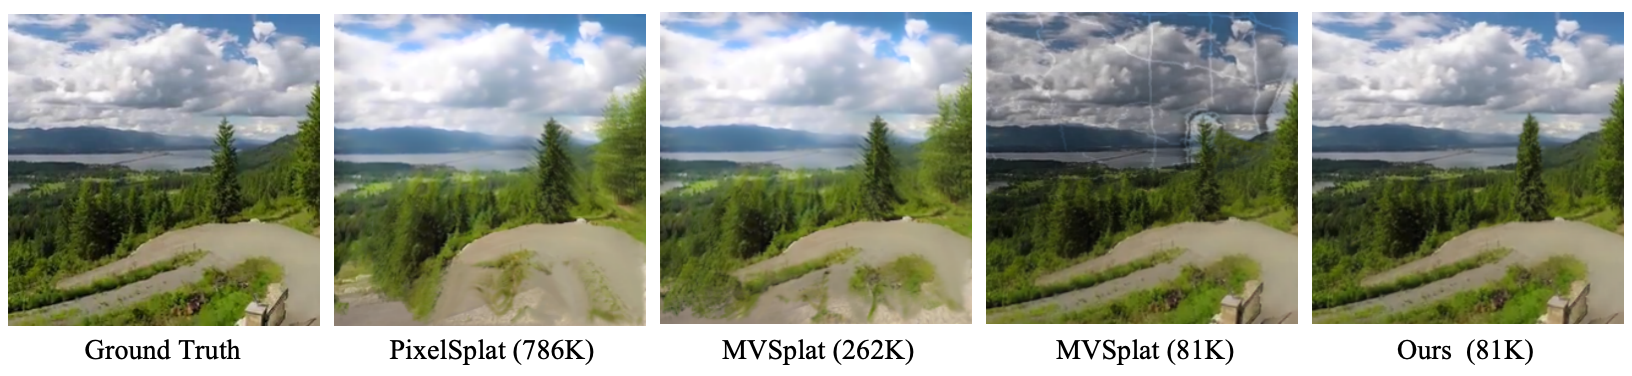
\includegraphics[height=0.22\linewidth]{fig/teaser_1.png}}
  \vspace{-0.2cm}
  \begin{minipage}[h]{0.99\linewidth}
      \centering            
      \subfloat[]{{\label{fig:teaser_2}}   
      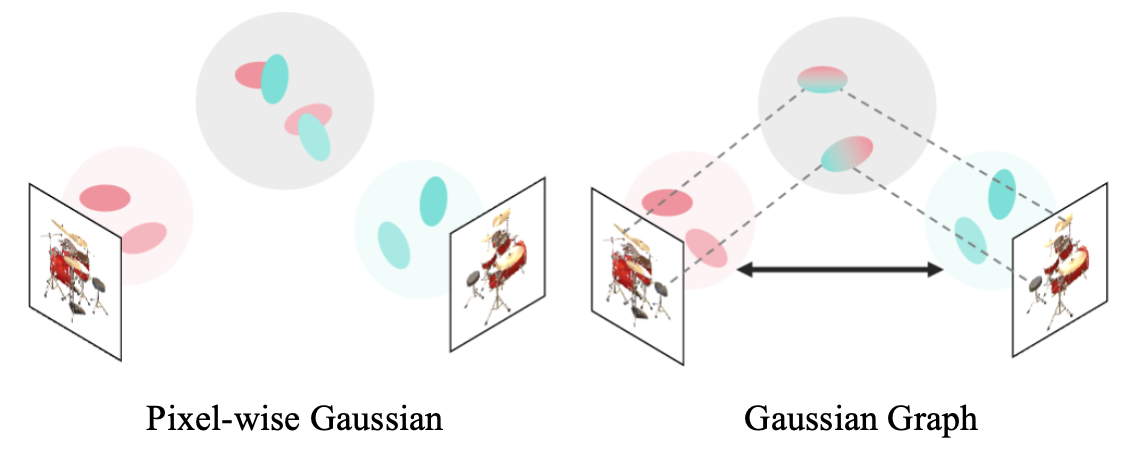
\includegraphics[height=0.26\linewidth]{fig/teaser_2.png}}
      \subfloat[]{{\label{fig:teaser_3}}
      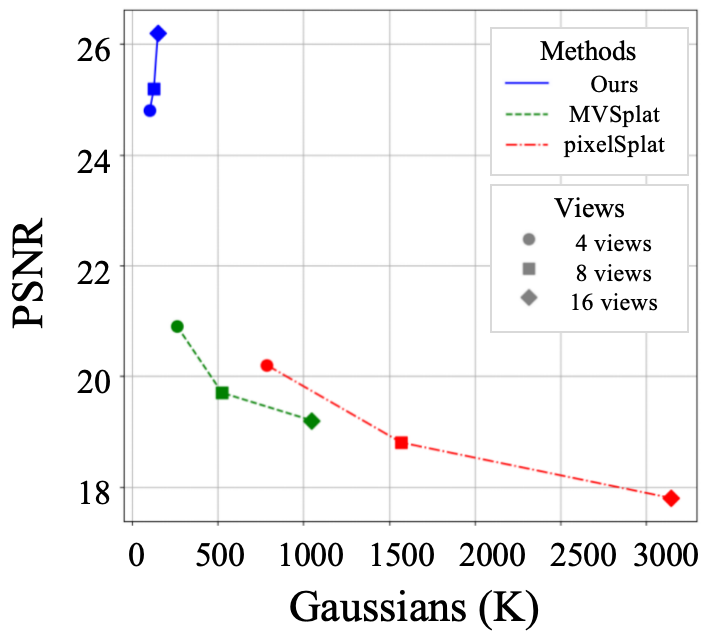
\includegraphics[height=0.26\linewidth]{fig/teaser_3.png}}
  \end{minipage}
  \caption{Comparison of previous methods and ours. (a) We visualize the rendering results of various methods and report the number of Gaussians in parentheses. (b) Previous pixel-wise methods can be considered as a degraded case of Gaussian Graphs without edges. (c) We report PSNR as well as the number of Gaussians for pixelSplat~\cite{pixelSplat2023arXiv}, MVSplat~\cite{MVSplat2024arXiv} and GNN under different input settings.}
  \label{fig:teaser}
  \vspace{-0.2cm}
\end{figure}
    

\section{Related Works}
\label{sec:related}
\subsection{Encoder-based MLLMs}
The dominant architecture of MLLMs has remained largely unchanged since its inception, comprising three components: a ViT \cite{clip, siglip, aimv2}, an LLM \cite{llama, gpt3, qwen2.5, vicuna}, and a connector to bridge modality gaps. Previous research has focused primarily on connector design, ranging from simple MLP layers \cite{llava, llava1_5, minigpt, minigptv2} to hierarchical feature fusion modules \cite{flamingo, llama3.2} or other complex architectures \cite{elysium, dynamicvlm, internvl, cambrian1}. Despite these innovations, fundamental limitations persist due to their reliance on external vision encoders. First, computational and memory overhead escalates dramatically when applying multiple vision encoders \cite{cambrian1} or scaling to larger ones \cite{cogvlm}. Second, fixed-resolution pre-training of ViTs forces MLLMs to employ workarounds like image tiling \cite{llava1_5, llavaov} or restricted square resolutions \cite{cogvlm, qwen}. Recent attempts \cite{pixtral, qwen2vl, aimv2} to train resolution-agnostic ViTs have remained impractical, in that they adopted massive proprietary data and opaque training procedures. These challenges have spurred interest in encoder-free architectures that could bypass ViTs entirely.
\subsection{Encoder-free MLLMs}
The pioneering work, Fuyu \cite{fuyu}, demonstrated the feasibility of training encoder-free models on interleaved image-text data, though at prohibitive computational costs with limited technical transparency. Subsequent approaches, such as EVE \cite{eve}, reduced the vision encoder parameters to a single Transformer block, aligning its output features with a ViT through distillation while updating all LLM parameters to learn about vision during the main training stage. However, these methods still struggle with conflicts between the LLM’s inherent language abilities and the new modality, i.e., vision. These conflicts arise from the coupled language and vision parameters, which exacerbate unstable training and lead to catastrophic forgetting of the original language abilities.
% Fuyu \cite{fuyu} pioneered such an approach by training on interleaved image-text data. However, this method required substantial computational resources and the detailed technic is unavalable. Subsequent efforts, such as EVE \cite{eve}, explored converting pre-trained LLMs into MLLMs by replacing ViTs with a single transformer block and aligning features via a distillation-like method. This can be understood as reducing the parameters of the vision encoder. During their main stage training, all LLM parameters are updated. Such methods have certain issues, where the modality confliction between a well-pretrained LLM and a new modality that LLM has never seen before remains a severe problem that can easily cause the training unstable, and even we can stablize the training, such method suffer from catastropic forgetting issue.

To overcome these problems, Mono-InternVL \cite{monointernvl} and EVEv2 \cite{evev2} proposed parameter decoupling strategies inspired by the MoE method \cite{moe}, duplicating LLM parameters for vision-specific processing while freezing its original weights. Despite successfully addressing forgetting issues and modality conflicts, these methods suffered from substantial memory overhead by doubling model parameters, compromising architectural simplicity. 
% This tension highlights a critical insight: preserving LLM integrity while integrating vision understanding requires strict parameter decoupling without persistent duplication. 
Our work addresses this by applying LoRA, which encodes vision while maintaining the language abilities of the LLM, and can be merged into the LLM without causing additional memory overhead.
%while maintaining modality alignment.


% \subsection{Encoder-based MLLM}
% The mainstream architecture of MLLMs follows the “Vision-Connector-LLM” framework, consisting of three key components: the vision encoder(s), the connector, and the LLM. Below, we examine these components in detail.
% \\
% \textbf{vision Encoder}
% The vision encoders used in MLLMs are often trained with contrastive learning loss on image-text tasks, such as CLIP. Additionally, there are other vision encoders trained on vision tasks using self-supervised or semi-supervised objectives. These pre-trained vision encoders provide strong prior knowledge in vision, making them widely adopted in MLLMs.
% \\
% \textbf{Connector}
% Due to the misalignment between the semantic spaces of vision encoders and LLMs, a connector is typically required to bridge this gap, which is one of the most distinctive functions of the connector. Its architecture can vary based on its additional functions, such as re-sampling to reduce the number of visual tokens.
% \\
% \textbf{LLM}
% The LLM often serves as the core component of the architecture, consuming the majority of computations and parameters. These models are typically developed by large companies or organizations due to the substantial amounts of data and training costs involved. The open community usually focuses on post-training enhancements or develops MLLMs based on existing LLMs.
% \subsection{\mono}
% We define \mono as utilizing a single Transformer, specifically an LLM, to perform multimodal tasks. This architecture requires only a few parameters to convert the dimensionality of data from other modalities, such as using a patchifier for vision, without the need for additional pre-trained models. The explorations of this kind of architecture emerges quite early, but soon struggles in several problems caused by the big gap between 
\section{Method}
\label{sec:method}
Our approach, in line with previous methods, builds upon a pre-trained VLM, CLIP \cite{clip}. In this section, we detail the construction of our MMRL framework and the implementation specifics.

\subsection{Preliminary}
We begin by defining the notations used in our approach. CLIP comprises two encoders: an image encoder $\mathcal{V}$ and a text encoder $\mathcal{W}$.

\noindent \textbf{Image Encoding:} The image encoder $\mathcal{V}$ consists of $L$ transformer \cite{transformer} layers, denoted $\{\mathcal{V}_i\}_{i=1}^{L}$. Given an input image \( x \in \mathbb{R}^{H \times W \times 3} \), it is divided into \( M \) fixed-size patches, each projected into a patch embedding, resulting in \( E_0 \in \mathbb{R}^{M \times d_v} \), where $M$ represents the number of patches and $d_v$ the embedding dimension. The initial patch embeddings $E_0$ are combined with a learnable class token $c_0$ and positional encodings, forming the input sequence for the transformer layers. Each layer processes this sequence as
\begin{equation}
    [c_i, E_i] = \mathcal{V}_i([c_{i-1}, E_{i-1}]) \quad
    i = 1, 2, \ldots, L
    \nonumber
\end{equation}
After passing through all transformer layers, a patch projection layer, $P_v^c$, projects the output of the class token, $c_L$, into a shared V-L latent space,
\begin{equation}
    f = P_v^c(c_L)
    \nonumber
\end{equation}
where $f \in \mathbb{R}^{d}$.

\noindent \textbf{Text Encoding:} For an input text, \eg, ``A photo of a [CLASS].", it is tokenized and converted into embeddings $T_0 \in \mathbb{R}^{N \times d_t}$, where $N$ is the token length and $d_t$ the embedding dimension. Beginning-of-text (BOT) and end-of-text (EOT) tokens, denoted $b_0$ and $e_0$, mark the sequence boundaries. These token embeddings, with positional encodings, are passed through the text encoder's $L$ transformer layers, $\{\mathcal{W}_i\}_{i=1}^{L}$, as follows,
\begin{equation} 
    [b_i, T_i, e_i] = \mathcal{W}_i([b_{i-1}, T_{i-1}, e_{i-1}]) \quad i = 1, \ldots, L 
    \nonumber
\end{equation} 
After the final layer, the output of the EOT token, $e_L$, is projected into the shared V-L space using $P_t$,
\begin{equation} 
    w = P_{t}(e_{L}) \nonumber
\end{equation} 
where $w \in \mathbb{R}^{d}$.

\noindent \textbf{Classification with CLIP:} With the image feature $f$ and text features $\{w_c\}_{c=1}^C$ for $C$ classes, CLIP calculates the cosine similarity between $f$ and each $w_c$,
\begin{equation} 
    \text{sim}(f, w_c) = \frac{f \cdot w_c}{|f| |w_c|}, \nonumber 
\end{equation} 
where $|\cdot|$ represents the $L_2$ norm. Class probabilities are then computed using the softmax function,
\begin{equation} 
    p(y = c \mid f) = \frac{\exp(\text{sim}(f, w_c) / \tau)}{\sum_{i=1}^{C} \exp(\text{sim}(f, w_i) / \tau)} \nonumber 
\end{equation} 
where $\tau$ is a temperature parameter. The final predicted class is selected as the one with the highest probability score.

% The predicted class $\hat{y}$ is determined by: \begin{equation} 
%     \hat{y} = \arg\max_{c} , p(y = c \mid f). \nonumber
% \end{equation}


%-------------------------------------------------------------------------
\begin{figure*}[tb]
\setlength{\abovecaptionskip}{0.2cm}   %调整图片标题与图距离
\setlength{\belowcaptionskip}{-0.4cm}   %调整图片标题与下文距离
\centering
\setlength{\belowcaptionskip}{-0.39cm}   %调整图片标题与下文距离
  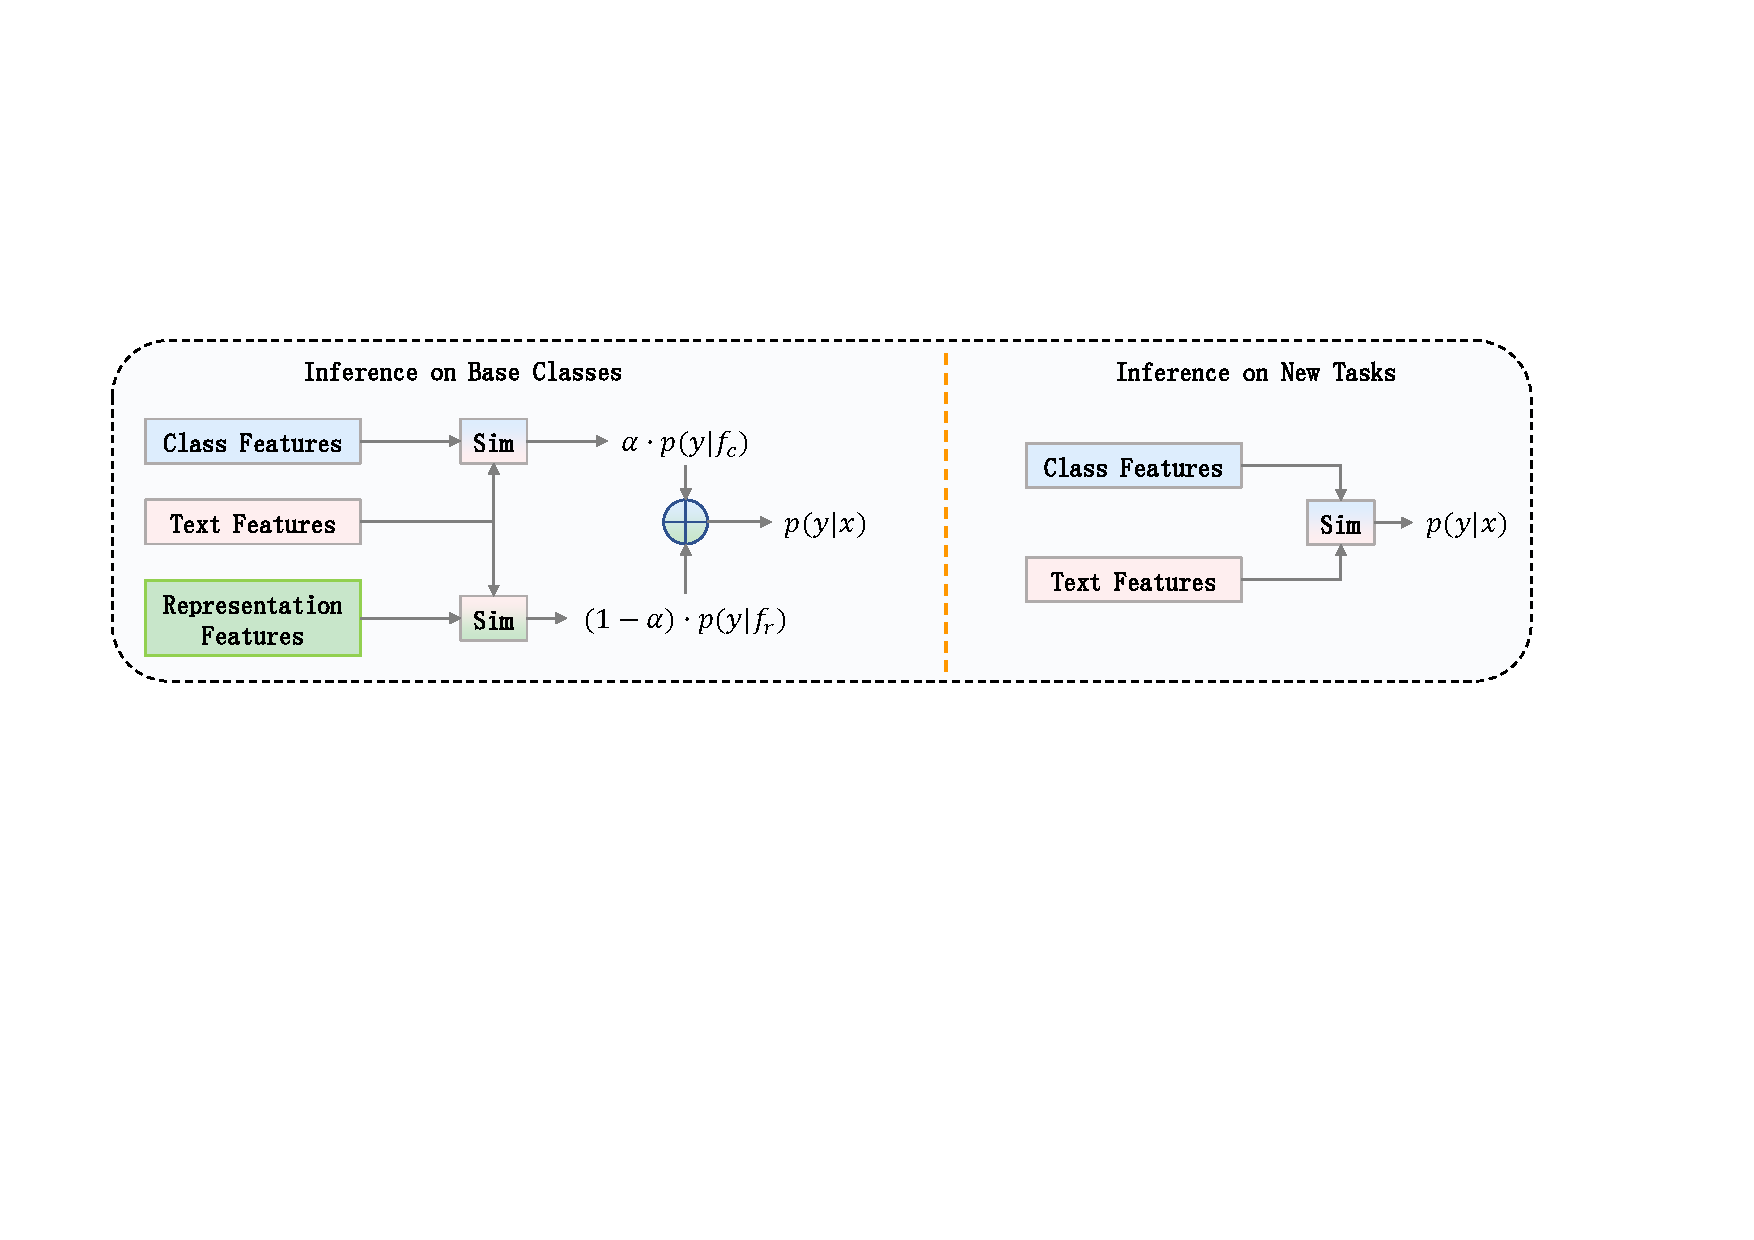
\includegraphics[width=0.7\linewidth]{fig/frame2.pdf}
  \caption{MMRL inference process, where different tasks utilize distinct features.}
  \label{framework2}
\end{figure*}
%-------------------------------------------------------------------------


\subsection{Multi-Modal Representation Learning (MMRL)} Our proposed MMRL aims to address the challenges of adapting pre-trained VLMs using few-shot data while maintaining generalization to new tasks. The training and inference frameworks of MMRL are shown in \cref{framework1} and \cref{framework2}, respectively. In the following, we describe the specifics of the methodology.


\subsubsection{Learnable Representation Space}
MMRL establishes a shared, learnable representation space $\mathcal{R}$ to facilitate multimodal interactions, initialized through sampling from a Gaussian distribution. Using a learnable mapping function $\mathcal{F}(\cdot)$, implemented as a linear layer, we project the tokens $R \in \mathbb{R}^{K \times d_r}$ in this space—where $K$ is the number of tokens and $d_r$ is the dimension of the representation space—into both visual and textual modalities,
\begin{align}
    R^v = \{R_i^v\}_{i=J-1}^{L-1} \quad & R_i^v = \mathcal{F}_i^v(R) \nonumber \\ 
    R^t = \{R_i^t\}_{i=J-1}^{L-1} \quad & R_i^t = \mathcal{F}_i^t(R) \nonumber 
\end{align}
where $R_i^v \in \mathbb{R}^{K \times d_v}$ and $R_i^t \in \mathbb{R}^{K \times d_t}$ represent the representation tokens for visual and textual modalities, respectively, in the $(i+1)$-th transformer layer. The index $J$ indicates the starting layer from which these representation tokens are integrated into the encoders.


\subsubsection{Integration into Higher Encoder Layers}
To preserve the generalized knowledge in the lower layers of the pre-trained CLIP model, the representation tokens $\mathcal{R}^v$ and $\mathcal{R}^t$ are integrated into the higher layers of the image encoder $\mathcal{V}$ and the text encoder $\mathcal{W}$, beginning from the $J$-th layer.


For the image encoder $\mathcal{V}$,
\begin{align}
    [c_i, E_i] &= \mathcal{V}_i([c_{i-1}, E_{i-1}]) \quad i = 1, \ldots, J-1 \nonumber \\  
    [c_i, \_, E_i] &= \mathcal{V}_i([c_{i-1}, R_{i-1}^v, E_{i-1}]) \quad i = J, \ldots, L - 1 \nonumber \\
    [c_i, R_i^v, E_i] &= \mathcal{V}_i([c_{i-1}, R_{i-1}^v, E_{i-1}]) \quad i = L \nonumber
\end{align}

For the text encoder $\mathcal{W}$, while previous prompt learning \cite{maple} involves replacing parts of $T_i$ to incorporate deep prompts, we retain the entire $T_i$ and insert $R_i^t$ before it, aiming to preserve the original textual information,
\begin{align}
    [b_i, T_i, e_i] &= \mathcal{W}_i([b_{i-1}, T_{i-1}, e_{i-1}]) \quad i = 1, \ldots, J-1 \nonumber \\  
    [b_i, \_, T_i, e_i] &= \mathcal{W}_i([b_{i-1}, R_{i-1}^t, T_{i-1}, e_{i-1}]) \nonumber \\
    &\hspace{4cm} i = J, \ldots, L-1 \nonumber \\
    [b_i, R_i^t, T_i, e_i] &= \mathcal{W}_i([b_{i-1}, R_{i-1}^t, T_{i-1}, e_{i-1}]) \quad i = L \nonumber
\end{align}
Note that due to the autoregressive nature of the text encoder, we adjust the attention mask matrix to accommodate the increased embedding length.


\subsubsection{Representation Learning}
Representation learning is designed to leverage representation tokens for dataset-specific adaptation, while the class token preserves the pre-trained knowledge of the original CLIP. Through a set of strategies aimed at retaining generalization during both training and inference, MMRL enables flexible inference for different tasks, as detailed below.


\begin{itemize} 

\item \textbf{Training Phase:} We optimize the features of both the representation tokens and the original class token, with the primary focus on representation features to preserve pre-trained knowledge. Specifically, the projection layer for the representation tokens is trainable, while that for the class token remains fixed. For the image encoder $\mathcal{V}$, after passing through $L$ transformer layers, we obtain the output $c_L \in \mathbb{R}^{d_v}$ for the class token and $R_L^v \in \mathbb{R}^{K \times d_v}$ for the $K$ representation tokens. The final output of the representation tokens, $r_L$, is derived by averaging across the $K$ tokens,
\begin{equation}
    r_L = \text{Mean}(R_L^v) \nonumber
\end{equation}
where $r_L \in \mathbb{R}^{d_v}$. We then apply the patch projection layers to map the outputs of both the class and representation tokens into the common V-L latent space, yielding the class features $f_c$ and representation features $f_r$.
\begin{equation}
    f_c = P_v^c(c_L) \quad f_r = P_v^r(r_L) \nonumber
\end{equation}
Here, $P_v^c$ is the original, frozen patch projection layer of CLIP for class features, while $P_v^r$ for representation features is trainable.

For the text encoder $\mathcal{W}$, following the sequential nature of text, we map the EOT token $e_L$—as in the original CLIP model—after processing through $L$ transformer layers into the common V-L space, yielding the text features.
\begin{equation} 
    w = P_{t}(e_{L}) \nonumber
\end{equation}
With the image features $f_c$, $f_r$, and the text classifiers $\{w_c\}_{c=1}^C$ for $C$ classes, we apply cross-entropy loss to separately optimize the class and representation features,
\begin{align}
\setlength\abovedisplayskip{3pt}
\setlength\belowdisplayskip{3pt}
    \mathcal{L}_{ce}^c &= -\sum_c^C y_c \log p(y = c \mid f_c) \nonumber \\
    \mathcal{L}_{ce}^r &= -\sum_c^C y_c \log p(y = c \mid f_r) \nonumber
\end{align}
where $y_c = 1$ if the image $x$ belongs to class $c$, and $y_c = 0$ otherwise. To further preserve the generalization of class features, we maximize the cosine similarity between $(f_c, w)$ and the frozen CLIP features $(f_0, w_0)$, explicitly guiding the training trajectory,
\begin{equation}
    \mathcal{L}_{cos}^v = 1 - \frac{f_c \cdot f_0}{|f_c| |f_0|} \quad \mathcal{L}_{cos}^t = 1 - \frac{1}{C}\sum_c^C \frac{w^c \cdot w_0^c}{|w^c| |w_0^c|}, \nonumber
\end{equation}
The final MMRL loss function is
\begin{equation}
    \mathcal{L}_{MMRL} = \alpha \mathcal{L}_{ce}^c + (1 - \alpha) \mathcal{L}_{ce}^r + \lambda (\mathcal{L}_{cos}^v + \mathcal{L}_{cos}^t)  \nonumber
\end{equation}
where $\alpha$ controls the balance between the features, and $\lambda$ is the penalty coefficient.

\item \textbf{Testing on Base Classes:} 
For in-distribution classes seen during training, we combine the dataset-specific representation features with the class features that preserve generalizability. The probability of an in-distribution test sample $x$ belonging to the $c$-th class is
\begin{equation}
    p(y = c \mid x) = \alpha \cdot p(y = c \mid f_c) + (1-\alpha) \cdot p(y = c \mid f_r) \nonumber
\end{equation}
where $f_c$ and $f_r$ are features extracted from the class token and representation tokens, respectively.

\item  \textbf{Testing on Novel Classes:}
For classes unseen during training or for new datasets, we rely solely on the class tokens, which retain generalized knowledge.
\begin{equation}
    p(y = c \mid x) = p(y = c \mid f_c) \nonumber
\end{equation}
\end{itemize}



% Then the predicted class $\hat{y}$ is determined by, 
% \begin{equation} 
%     \hat{y} = \arg\max_{c} , p(y = c \mid x). \nonumber
% \end{equation}



\begin{table*}[t]
\centering
\setlength{\abovecaptionskip}{0.15cm}   %调整表格标题与表格距离
\caption{Comparison of MMRL with previous state-of-the-art methods on base-to-novel generalization across 11 datasets. Bold values indicate the best results. MMRL consistently enhances base class performance without compromising generalization.}
\label{base_to_novel}
\renewcommand\arraystretch{1.06}
\setlength{\tabcolsep}{2.87mm}{
\resizebox{0.85\textwidth}{!}{
    \begin{tabular}{@{}r|ccc|ccc|ccc|ccc@{}}
    \toprule
    \multirow{2}{*}{Method} &
      \multicolumn{3}{c|}{Average} &
      \multicolumn{3}{c|}{ImageNet} &
      \multicolumn{3}{c|}{Caltech101} &
      \multicolumn{3}{c}{OxfordPets} \\
     &
      Base &
      Novel &
      HM &
      Base &
      Novel &
      HM &
      Base &
      Novel &
      HM &
      Base &
      Novel &
      HM \\ \midrule
    $\text{CLIP}_{\text{ (ICML2021)}}$ &
      69.34 &
      74.22 &
      71.70 &
      72.43 &
      68.14 &
      70.22 &
      96.84 &
      94.00 &
      95.40 &
      91.17 &
      97.26 &
      94.12 \\
    $\text{CoOp}_{\text{ (IJCV2022)}}$ &
      82.69 &
      63.22 &
      71.66 &
      76.47 &
      67.88 &
      71.92 &
      98.00 &
      89.81 &
      93.73 &
      93.67 &
      95.29 &
      94.47 \\
    $\text{CoOpOp}_{\text{ (CVPR2022)}}$ &
      80.47 &
      71.69 &
      75.83 &
      75.98 &
      70.43 &
      73.10 &
      97.96 &
      93.81 &
      95.84 &
      95.20 &
      97.69 &
      96.43 \\
    $\text{ProDA}_{\text{ (CVPR2022)}}$ &
      81.56 &
      72.30 &
      76.65 &
      75.40 &
      70.23 &
      72.72 &
      98.27 &
      93.23 &
      95.68 &
      95.43 &
      97.83 &
      96.62 \\
    $\text{KgCoOp}_{\text{ (CVPR2023)}}$ &
      80.73 &
      73.60 &
      77.00 &
      75.83 &
      69.96 &
      72.78 &
      97.72 &
      94.39 &
      96.03 &
      94.65 &
      97.76 &
      96.18 \\
    $\text{MaPLe}_{\text{ (CVPR2023)}}$ &
      82.28 &
      75.14 &
      78.55 &
      76.66 &
      70.54 &
      73.47 &
      97.74 &
      94.36 &
      96.02 &
      95.43 &
      97.76 &
      96.58 \\
    $\text{PromptSRC}_{\text{ (ICCV2023)}}$ &
      84.26 &
      76.10 &
      79.97 &
      77.60 &
      70.73 &
      74.01 &
      98.10 &
      94.03 &
      96.02 &
      95.33 &
      97.30 &
      96.30 \\
    $\text{ProVP}_{\text{ (IJCV2024)}}$ &
      85.20 &
      73.22 &
      78.76 &
      75.82 &
      69.21 &
      72.36 &
      98.92 &
      94.21 &
      96.51 &
      95.87 &
      97.65 &
      \textbf{96.75} \\
    $\text{MetaPrompt}_{\text{ (TIP2024)}}$ &
      83.65 &
      75.48 &
      79.09 &
      77.52 &
      70.83 &
      74.02 &
      98.13 &
      94.58 &
      96.32 &
      95.53 &
      97.00 &
      96.26 \\
    $\text{TCP}_{\text{ (CVPR2024)}}$ &
      84.13 &
      75.36 &
      79.51 &
      77.27 &
      69.87 &
      73.38 &
      98.23 &
      \textbf{94.67} &
      96.42 &
      94.67 &
      97.20 &
      95.92 \\
    $\text{MMA}_{\text{ (CVPR2024)}}$ &
      83.20 &
      76.80 &
      79.87 &
      77.31 &
      71.00 &
      74.02 &
      98.40 &
      94.00 &
      96.15 &
      95.40 &
      \textbf{98.07} &
      96.72 \\ \midrule
    $\text{MMRL}_{\text{ (Ours)}}$ &
      \textbf{85.68} &
      \textbf{77.16} &
      \textbf{81.20} &
      \textbf{77.90} &
      \textbf{71.30} &
      \textbf{74.45} &
      \textbf{98.97} &
      94.50 &
      \textbf{96.68} &
      \textbf{95.90} &
      97.60 &
      96.74 \\ \midrule \midrule
    \multirow{2}{*}{Method} &
      \multicolumn{3}{c|}{StanfordCars} &
      \multicolumn{3}{c|}{Flowers102} &
      \multicolumn{3}{c|}{Food101} &
      \multicolumn{3}{c}{FGVCAircraft} \\
     &
      Base &
      Novel &
      HM &
      Base &
      Novel &
      HM &
      Base &
      Novel &
      HM &
      Base &
      Novel &
      HM \\ \midrule
    $\text{CLIP}_{\text{ (ICML2021)}}$ &
      63.37 &
      74.89 &
      68.65 &
      72.08 &
      77.80 &
      74.83 &
      90.10 &
      91.22 &
      90.66 &
      27.19 &
      36.29 &
      31.09 \\
    $\text{CoOp}_{\text{ (IJCV2022)}}$ &
      78.12 &
      60.40 &
      68.13 &
      97.60 &
      59.67 &
      74.06 &
      88.33 &
      82.26 &
      85.19 &
      40.44 &
      22.30 &
      28.75 \\
    $\text{CoOpOp}_{\text{ (CVPR2022)}}$ &
      70.49 &
      73.59 &
      72.01 &
      94.87 &
      71.75 &
      81.71 &
      90.70 &
      91.29 &
      90.99 &
      33.41 &
      23.71 &
      27.74 \\
    $\text{ProDA}_{\text{ (CVPR2022)}}$ &
      74.70 &
      71.20 &
      72.91 &
      97.70 &
      68.68 &
      80.66 &
      90.30 &
      88.57 &
      89.43 &
      36.90 &
      34.13 &
      35.46 \\
    $\text{KgCoOp}_{\text{ (CVPR2023)}}$ &
      71.76 &
      75.04 &
      73.36 &
      95.00 &
      74.73 &
      83.65 &
      90.50 &
      91.70 &
      91.09 &
      36.21 &
      33.55 &
      34.83 \\
    $\text{MaPLe}_{\text{ (CVPR2023)}}$ &
      72.94 &
      74.00 &
      73.47 &
      95.92 &
      72.46 &
      82.56 &
      90.71 &
      \textbf{92.05} &
      \textbf{91.38} &
      37.44 &
      35.61 &
      36.50 \\
    $\text{PromptSRC}_{\text{ (ICCV2023)}}$ &
      78.27 &
      74.97 &
      76.58 &
      98.07 &
      76.50 &
      85.95 &
      90.67 &
      91.53 &
      91.10 &
      42.73 &
      \textbf{37.87} &
      40.15 \\
    $\text{ProVP}_{\text{ (IJCV2024)}}$ &
      80.43 &
      67.96 &
      73.67 &
      98.42 &
      72.06 &
      83.20 &
      90.32 &
      90.91 &
      90.61 &
      \textbf{47.08} &
      29.87 &
      36.55 \\
    $\text{MetaPrompt}_{\text{ (TIP2024)}}$ &
      76.34 &
      75.01 &
      75.48 &
      97.66 &
      74.49 &
      84.52 &
      \textbf{90.74} &
      91.85 &
      91.29 &
      40.14 &
      36.51 &
      38.24 \\
    $\text{TCP}_{\text{ (CVPR2024)}}$ &
      80.80 &
      74.13 &
      77.32 &
      97.73 &
      75.57 &
      85.23 &
      90.57 &
      91.37 &
      90.97 &
      41.97 &
      34.43 &
      37.83 \\
    $\text{MMA}_{\text{ (CVPR2024)}}$ &
      78.50 &
      73.10 &
      75.70 &
      97.77 &
      75.93 &
      85.48 &
      90.13 &
      91.30 &
      90.71 &
      40.57 &
      36.33 &
      38.33 \\ \midrule
    $\text{MMRL}_{\text{ (Ours)}}$ &
      \textbf{81.30} &
      \textbf{75.07} &
      \textbf{78.06} &
      \textbf{98.97} &
      \textbf{77.27} &
      \textbf{86.78} &
      90.57 &
      91.50 &
      91.03 &
      46.30 &
      37.03 &
      \textbf{41.15} \\ \midrule \midrule
    \multirow{2}{*}{Method} &
      \multicolumn{3}{c|}{SUN397} &
      \multicolumn{3}{c|}{DTD} &
      \multicolumn{3}{c|}{EuroSAT} &
      \multicolumn{3}{c}{UCF101} \\
     &
      Base &
      Novel &
      HM &
      Base &
      Novel &
      HM &
      Base &
      Novel &
      HM &
      Base &
      Novel &
      HM \\ \midrule
    $\text{CLIP}_{\text{ (ICML2021)}}$ &
      69.36 &
      75.35 &
      72.23 &
      53.24 &
      59.90 &
      56.37 &
      56.48 &
      64.05 &
      60.03 &
      70.53 &
      77.50 &
      73.85 \\
    $\text{CoOp}_{\text{ (IJCV2022)}}$ &
      80.60 &
      65.89 &
      72.51 &
      79.44 &
      41.18 &
      54.24 &
      92.19 &
      54.74 &
      68.69 &
      84.69 &
      56.05 &
      67.46 \\
    $\text{CoOpOp}_{\text{ (CVPR2022)}}$ &
      79.74 &
      76.86 &
      78.27 &
      77.01 &
      56.00 &
      64.85 &
      87.49 &
      60.04 &
      71.21 &
      82.33 &
      73.45 &
      77.64 \\
    $\text{ProDA}_{\text{ (CVPR2022)}}$ &
      78.67 &
      76.93 &
      77.79 &
      80.67 &
      56.48 &
      66.44 &
      83.90 &
      66.00 &
      73.88 &
      85.23 &
      71.97 &
      78.04 \\
    $\text{KgCoOp}_{\text{ (CVPR2023)}}$ &
      80.29 &
      76.53 &
      78.36 &
      77.55 &
      54.99 &
      64.35 &
      85.64 &
      64.34 &
      73.48 &
      82.89 &
      76.67 &
      79.65 \\
    $\text{MaPLe}_{\text{ (CVPR2023)}}$ &
      80.82 &
      78.70 &
      79.75 &
      80.36 &
      59.18 &
      68.16 &
      94.07 &
      73.23 &
      82.35 &
      83.00 &
      78.66 &
      80.77 \\
    $\text{PromptSRC}_{\text{ (ICCV2023)}}$ &
      82.67 &
      78.47 &
      80.52 &
      83.37 &
      62.97 &
      71.75 &
      92.90 &
      73.90 &
      82.32 &
      87.10 &
      78.80 &
      82.74 \\
    $\text{ProVP}_{\text{ (IJCV2024)}}$ &
      80.67 &
      76.11 &
      78.32 &
      83.95 &
      59.06 &
      69.34 &
      \textbf{97.12} &
      72.91 &
      83.29 &
      \textbf{88.56} &
      75.55 &
      81.54 \\
    $\text{MetaPrompt}_{\text{ (TIP2024)}}$ &
      82.26 &
      79.04 &
      80.62 &
      83.10 &
      58.05 &
      68.35 &
      93.53 &
      75.21 &
      83.38 &
      85.33 &
      77.72 &
      81.35 \\
    $\text{TCP}_{\text{ (CVPR2024)}}$ &
      82.63 &
      78.20 &
      80.35 &
      82.77 &
      58.07 &
      68.25 &
      91.63 &
      74.73 &
      82.32 &
      87.13 &
      \textbf{80.77} &
      83.83 \\
    $\text{MMA}_{\text{ (CVPR2024)}}$ &
      82.27 &
      78.57 &
      80.38 &
      83.20 &
      \textbf{65.63} &
      73.38 &
      85.46 &
      \textbf{82.34} &
      83.87 &
      86.23 &
      80.03 &
      82.20 \\ \midrule
    $\text{MMRL}_{\text{ (Ours)}}$ &
      \textbf{83.20} &
      \textbf{79.30} &
      \textbf{81.20} &
      \textbf{85.67} &
      65.00 &
      \textbf{73.82} &
      95.60 &
      80.17 &
      \textbf{87.21} &
      88.10 &
      80.07 &
      \textbf{83.89} \\ \bottomrule
    \end{tabular}
            }
}
\vspace{-0.3cm}
\end{table*}







\begin{table*}[ht]
\centering
\small
\renewcommand{\arraystretch}{0.95}
\renewcommand\tabcolsep{4pt}
\begin{tabular}{cc|c|c|c|c|ccc}
\hline 
\multicolumn{2}{c|}{Dataset} & Model & Venue & Base & Method & mAP$\uparrow$ & Rank-1$\uparrow$ & $\text{ID}^2$$\downarrow$ \\ \hline
% \multicolumn{2}{c|}{} & & & & ori & 3.34 & 11.4 & 0.5135 \\ \cline{6-9} 
% \multicolumn{2}{c|}{} & \multirow{-2}{*}{TransReID\cite{he2021transreid}(w/o training)} & & & +ours & 52.81\scriptsize{(+49.47)} & 78.92\scriptsize{(+67.52)} & 0.2158 \\ \cline{3-3} \cline{6-9} 
\multicolumn{2}{c|}{} & & & & official & 79.88 & 91.48 & 0.2193 \\ \cline{6-9} 
\multicolumn{2}{c|}{} & \multirow{-2}{*}{TransReID\cite{he2021transreid}(w/o camid)} & & & +ours & 90.39\scriptsize{(+10.51)} & 94.74\scriptsize{(+3.26)} & 0.1357 \\ \cline{3-3} \cline{6-9} 
\multicolumn{2}{c|}{} & & & & official & 89 & 95.1 & 0.2759 \\ \cline{6-9} 
\multicolumn{2}{c|}{} & \multirow{-2}{*}{TransReID\cite{he2021transreid}(w/ camid)} & \multirow{-4}{*}{ICCV21} & \multirow{-4}{*}{ViT} & +ours & 93.01\scriptsize{(+4.01)} & 95.52\scriptsize{(+0.42)} & 0.1967 \\ \cline{3-9} 
\multicolumn{2}{c|}{} & & & & official & 89.7 & 95.4 & 0.0993 \\ \cline{6-9} 
\multicolumn{2}{c|}{} & & & \multirow{-2}{*}{ViT} & +ours & 94\scriptsize{(+4.3)} & 96.4\scriptsize{(+1.0)} & 0.0624 \\ \cline{5-9} 
\multicolumn{2}{c|}{} & & & & official & 89.8 & 95.7 & 0.0877 \\ \cline{6-9} 
\multicolumn{2}{c|}{\multirow{-8}{*}{Market1501}} & \multirow{-4}{*}{CLIP-ReID\cite{li2023clip}} & \multirow{-4}{*}{AAAI23} & \multirow{-2}{*}{CNN} & \cellcolor{gray!20}+ours & \cellcolor{gray!20}94.9\scriptsize{(+5.1)} & \cellcolor{gray!20}97.3\scriptsize{(+1.6)} & \cellcolor{gray!20}0.053 \\ \hline
\multicolumn{2}{c|}{} & & & & official & 79.05 & 85.4 & 0.3124 \\ \cline{6-9} 
\multicolumn{2}{c|}{} & \multirow{-2}{*}{KPR\cite{somers2025keypoint}} & \multirow{-2}{*}{ECCV24} & \multirow{-2}{*}{ViT} & \cellcolor{gray!20}+ours & \cellcolor{gray!20}89.34\scriptsize{(+10.29)} & \cellcolor{gray!20}91\scriptsize{(+5.6)} & \cellcolor{gray!20}0.1434 \\ \cline{3-9} 
\multicolumn{2}{c|}{} & & & & official & 70.41 & 77.2 & 0.377 \\ \cline{6-9} 
\multicolumn{2}{c|}{\multirow{-4}{*}{Occluded-ReID}} & \multirow{-2}{*}{BPBReID\cite{somers2023body}} & \multirow{-2}{*}{WACV23} & \multirow{-2}{*}{ViT} & +ours & 86.05\scriptsize{(+15.64)} & 89.1\scriptsize{(+11.9)} & 0.1504 \\ \hline
\multicolumn{1}{c|}{} & & & & & official & 71.81 & 75.29 & 0.4817 \\ \cline{6-9} 
\multicolumn{1}{c|}{} & \multirow{-2}{*}{All} & & & & \cellcolor{gray!20}+ours & \cellcolor{gray!20}76.44\scriptsize{(+4.63)} & \cellcolor{gray!20}79.33\scriptsize{(+4.04)} & \cellcolor{gray!20}0.4072 \\ \cline{2-2} \cline{6-9} 
\multicolumn{1}{c|}{} & & & & & official & 84.6 & 81.59 & 0.4424 \\ \cline{6-9} 
\multicolumn{1}{c|}{} & \multirow{-2}{*}{Indoor} & \multirow{-4}{*}{SAAI\cite{fang2023visible}} & \multirow{-4}{*}{ICCV23} & \multirow{-4}{*}{CNN} & \cellcolor{gray!20}+ours & \cellcolor{gray!20}86.83\scriptsize{(+2.23)} & \cellcolor{gray!20}84.2\scriptsize{(+2.61)} & \cellcolor{gray!20}0.3694 \\ \cline{2-9} 
\multicolumn{1}{c|}{} & & & & & official & 66.13 & 67.7 & 0.4308 \\ \cline{6-9} 
\multicolumn{1}{c|}{} & \multirow{-2}{*}{All} & & & & +ours & 75.43\scriptsize{(+9.3)} & 74.81\scriptsize{(+7.11)} & 0.3133 \\ \cline{2-2} \cline{6-9} 
\multicolumn{1}{c|}{} & & & & & official & 77.81 & 72.95 & 0.4046 \\ \cline{6-9} 
\multicolumn{1}{c|}{\multirow{-8}{*}{SYSU-MM01}} & \multirow{-2}{*}{Indoor} & \multirow{-4}{*}{PMT\cite{lu2023learning}} & \multirow{-4}{*}{AAAI23} & \multirow{-4}{*}{ViT} & +ours & 84.29\scriptsize{(+6.48)} & 80.29\scriptsize{(+7.34)} & 0.2995 \\ \hline
\end{tabular}

\caption{Improvements with our method on different SOTA models with both ViT and CNN backbone on Market1501, SYSU-MM01, and Occluded-ReID datasets. The data under \colorbox{gray!20}{grey} is the new SOTA with our methods of that dataset.}
\label{tab:sota}
\end{table*}


\begin{table*}[ht]
\centering
\small
\renewcommand{\arraystretch}{1.0}
\renewcommand\tabcolsep{4pt}
\begin{minipage}{0.32\textwidth}
\centering
\begin{tabular}{c|ccc}
\hline
\textbf{Methods} & mAP$\uparrow$ & Rank-1$\uparrow$ & $\text{ID}^2$$\downarrow$ \\ \hline
Base & 79.88 & 91.48 & 0.2193 \\
+NFC & 83.92 & 91.83 & 0.1824 \\
+IPG & 88.02 & 94.77 & 0.1553 \\
\rowcolor{gray!20}
+NFC+IPG & 90.39 & 94.74 & 0.1357 \\
\hline
\end{tabular}
\caption{Ablation study on effects of feature centralization through Identity-Guided Pedestrian Generation (IPG) and Neighbor Feature Centralization (NFC).}
\label{tab:ablation_fe_pg}
\end{minipage}
\hfill
\begin{minipage}{0.32\textwidth}
\centering
\begin{tabular}{cc|cc}
\hline
$\text{Gallery}^\text{NFC}$ & $\text{Query}^\text{NFC}$  & mAP$\uparrow$ & Rank-1$\uparrow$ \\ \hline
 \ding{55} & \ding{55}   & 79.88&	91.48  \\
 \ding{51} & \ding{55}    & 81.70 & 92.04  \\
\ding{55} & \ding{51}    & 82.76 & 91.69  \\
\rowcolor{gray!20}
\ding{51} & \ding{51}    & 83.92 & 91.83 \\ 
\hline
\end{tabular}
\caption{Ablation study of Neighbor Feature Centralization (NFC) Algorithm on Market1501 dataset. We test on the gallery and query set respectively.}
\label{tab:as_fe}
\end{minipage}
\hfill
\begin{minipage}{0.32\textwidth}
\centering
\begin{tabular}{cc|cc}
\hline
% \multicolumn{2}{c|}{\textbf{Methods}}& \multicolumn{4}{c}{Metrics}  \\ \hline
$\text{Gallery}^\text{IPG}$ & $\text{Query}^\text{IPG}$  & mAP$\uparrow$ & Rank-1$\uparrow$ \\ \hline
\ding{55} & \ding{55}   & 79.88&	91.48  \\
% \ding{51} & \ding{55}    &  84.06 &91.48 \\
% \ding{55} & \ding{51}    & 81.01 &91.03  \\
% \rowcolor{gray!20}
% \ding{51} & \ding{51}    & 87.38& 94.63 \\ 
 \ding{51} & \ding{55}    & 84.65&	92.07  \\
\ding{55} & \ding{51}    & 82.18	&92.40  \\
\rowcolor{gray!20}
\ding{51} & \ding{51}    &88.02&	94.77 \\ 
\hline
\end{tabular}
\caption{Ablation study of Feature ID-Centralizing with Pedestrian Generation (IPG) on Market1501. We test on gallery and query set respectively.}
\label{tab:as_gen}
\end{minipage}
\end{table*}


\begin{table}
\small
    \centering
    \renewcommand{\arraystretch}{1}
    \renewcommand\tabcolsep{6pt}
    \begin{tabular}{c|ccccc}
        \hline
        \textbf{Method} & mAP$\uparrow$ & R1$\uparrow$ & R5$\uparrow$ & R10$\uparrow$ & $\text{ID}^2$$\downarrow$ \\ \hline
        w/o training & 3.34 & 11.4 & 21.88 & 28 & 0.5135 \\
        \rowcolor{gray!20}
        +IPG & 52.81 & 78.92 & 91.21 & 94.27 & 0.2158 \\
        \rowcolor{gray!20}
        +IPG+NFC & 57.27 & 82.39 & 90.17 & 92.81 & 0.1890 \\ \hline
    \end{tabular}
    \caption{ReID performance on Market1501 with only ImageNet pre-trained weights without ReID training. The distribution visualized in Fig.\ref{fig:noise_tsne}.}
    \label{tab:notraining}
\end{table}
\begin{figure}[H]
\centering
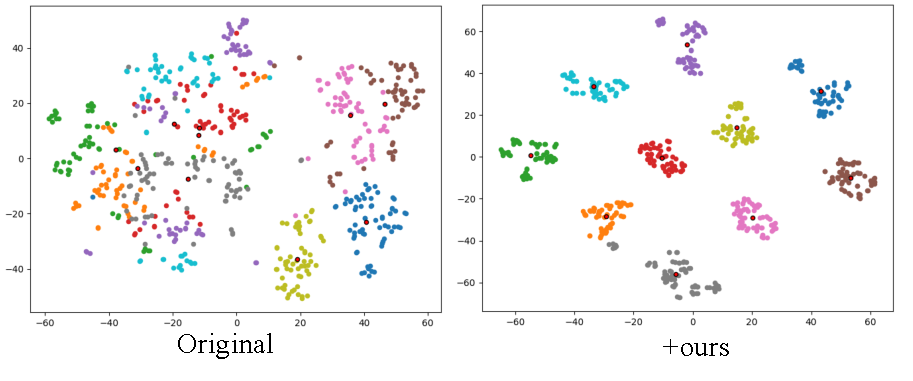
\includegraphics[width=0.95\linewidth]{figs/pdf/noise_tsne.pdf}
\caption{t-SNE visualization of 10 IDs feature distribution with and without our method on ImageNet pre-trained weights.}
\label{fig:noise_tsne}
\end{figure}


\section{Experiments}
\subsection{Implementation Details}

\textbf{Data Cleaning.}
Training an effective generative model requires high-quality data support. In current ReID (Person Re-Identification) datasets, there are many low-quality images, and removing them can help reduce interference to the model. In our experiments, we found two main issues that need to be addressed:\textbf{Extremely Low-quality Images}: The dataset contains images with such low resolution that even the human eye cannot recognize them as a "person". \textbf{Pose Estimation Failures}: The pose estimation model inevitably fails to detect pedestrian poses in some images.

Utilizing the feature distribution mentioned in Section\ref{Feature Distribution}, we can solve the issues and get the reference image set $S_i^{\text{ref}}$ and target image set $S^{\text{trg}}_i$ of identity $i$.
The cleansing process is detailed in \textbf{Supplementary}. 
\\
\textbf{Identity-guided Pedestrian Generation model details}
For the reference UNet and denoising UNet, we use the pretrained weights of Stable Diffusion v1.5\cite{rombach2022high}. The VAE encoder and decoder initialized with official weights\cite{kingma2013auto} and froze. For the ReID model, we use pre-trained TransReID\cite{he2021transreid} without cameras on Market1501 and freeze. 

The training data collected from training set of Market1501\cite{zheng2015scalable},  Mars\cite{zheng2016mars}, MSMT17\cite{wei2018person} and SYSU-MM01\cite{wu2017rgb}, with a total of 1946 different IDs. The model was trained for 80,000 iterations on one L20(48G) GPU with batch size of 4, which costs about 20 hours, and optimized by Adam\cite{kingma2014adam} with a learning rate of 1e-5 and weight decay of 0.01. All images are resized to 512×256. We applied random flip and random erasing\cite{zhong2020random} data augmentation only on reference images.

According to Section\ref{standard pose}, we selected 8 poses on the market1501 dataset as the representative poses. Each image in test set generates 8 images with these representative poses. The generation uses DDIM with 20 steps, classifier-free guidance with a scale of 3.5, and generator seed of 42.
\\
\textbf{ReID test settings}
Test models are loaded with official open-source pre-trained models for testing. In addition, considering the generated images do not have camera IDs, so for feature consistency, we test without camera IDs (e.g. TransReID). To validate the effectiveness of our proposed method, image flip (Section\ref{flip}) trick is \textbf{NOT} applied in our experiments. On Market1501, set \(\eta=2\), and \(k_1=k_2=2\). On Occluded REID, set \(\eta=1\), and \(k_1=k_2=1\). On SYSU-MM01, set \(\eta=1/4\), and \(k_1=k_2=2\). The parameters analysis detailed in \textbf{Supplementary}.



\subsection{Improvements on State-of-the-art Methods}
To verify the exceptional feature enhancement performance of our framework, we selected state-of-the-art models of three ReID tasks, divided into CNN and ViT-based models, to demonstrate that our theory can apply to any model and various ReID tasks. As shown in Table.\ref{tab:sota}, we achieved excellent enhancements on different models.

It is worth mentioning that we help models achieve new \textbf{SOTAs} without re-rank on 3 benchmarks:
\begin{itemize}
    \item[$\bullet$] \textbf{CNN-base CLIP-ReID on market1501: }
    
    \setlength{\parindent}{1em} mAP 94.9\%, Rank-1 97.3\%. 
    \item[$\bullet$] \textbf{KPR on Occluded-ReID: }

    \setlength{\parindent}{1em} mAP 89.34\%, Rank-1 91\%
    
    \item[$\bullet$] \textbf{SAAI on SYSU-MM01: }

    \setlength{\parindent}{1em} All-search mode: mAP 76.44\%, Rank-1 79.33\%
    
    \setlength{\parindent}{1em} Indoor-search mode: mAP 86.83\%, Rank-1 84.2\%
\end{itemize}



\subsection{ReID without Training}
TransReID loads a ViT pre-trained model on ImageNet for training on the ReID task. The pre-training method is based on contrastive learning strategies. According to the description in Section\ref{Feature Distribution}, training with contrastive loss helps to cluster features of same label samples. Images generated by our Pedestrian Generation model exhibit identity consistency, meaning they possess the attributes of the same label. Therefore, even if the features of an individual sample lack the pedestrian matching capability, as shown in the first row of Tab.\ref{tab:notraining}, its mAP and Rank-1 are only 3.34\% and 11.4\%. However, with our method, it improved 53.93\%/70.99\% to 57.27\%/82.39\%. Additionally, we visualized of 10 IDs' feature distributions using t-SNE as shown in Fig.\ref{fig:noise_tsne}.


\begin{figure}
\centering
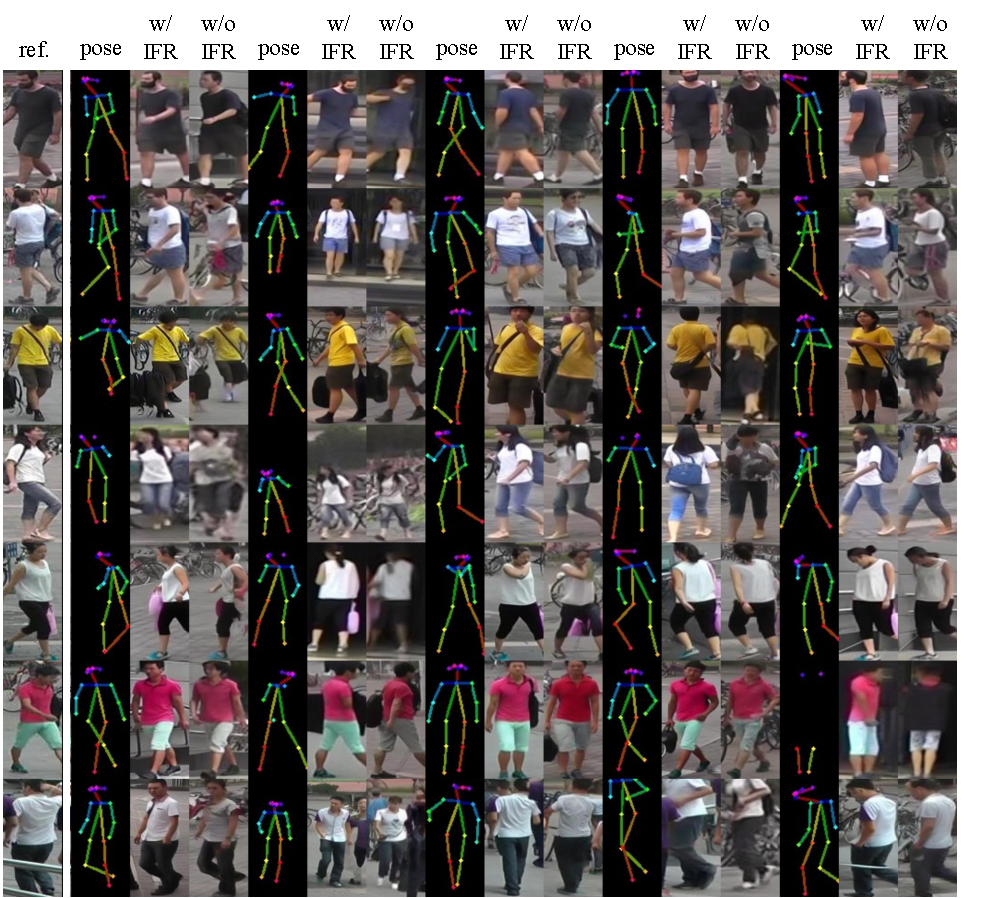
\includegraphics[width=0.95\linewidth]{figs/pdf/IFR.pdf}
\caption{The effects with and without the IFR module were visualized with five different poses randomly selected for each reference picture.}
\label{fig:IFR}
\end{figure}

\begin{table}
\small
    \centering
    \renewcommand{\arraystretch}{1}
    \renewcommand\tabcolsep{2pt}
    \begin{tabular}{c|ccc|ccc|ccc}
        \hline
        \multirow{2}{*}{\textbf{N}} & \multicolumn{3}{c|}{$\text{Gallery}^\text{IPG}$} & \multicolumn{3}{c|}{$\text{Query}^\text{IPG}$} & \multicolumn{3}{c}{$\text{Gallery}^\text{IPG}$+$\text{Query}^\text{IPG}$} \\ \cline{2-10}
          & mAP$\uparrow$ & R1$\uparrow$ & $\text{ID}^2$$\downarrow$ & mAP$\uparrow$ & R1$\uparrow$ & $\text{ID}^2$$\downarrow$ & mAP$\uparrow$ & R1$\uparrow$ & $\text{ID}^2$$\downarrow$ \\ \hline
        0 & 79.88 & 91.48 & 0.2313 & 79.88 & 91.48 & 0.1623 & 79.88 & 91.48 & 0.2193 \\
        1 & 80.96 & 90.97 & 0.2087 & 79.99 & 90.83 & 0.1363 & 82.13 & 92.01 & 0.1961 \\
        2 & 82.86 & 91.45 & 0.1904 & 81.17 & 92.04 & 0.1156 & 85.27 & 93.71 & 0.1773 \\
        3 & 83.42 & 91.75 & 0.1837 & 81.55 & 92.25 & 0.1077 & 86.16 & 94.21 & 0.1704 \\
        4 & 83.81 & 92.1  & 0.1795 & 81.76 & 92.34 & 0.1027 & 86.75 & 94.24 & 0.1661 \\
        5 & 84.07 & 91.83 & 0.1758 & 81.85 & 92.07 & 0.0984 & 87.23 & 94.71 & 0.1623 \\
        6 & 84.3  & 91.98 & 0.1730 & 81.96 & 92.52 & 0.0950 & 87.52 & 94.63 & 0.1593 \\
        7 & 84.49 & 91.86 & 0.1707 & 82.03 & 92.37 & 0.0922 & 87.76 & 94.60 & 0.1570 \\
        \rowcolor{gray!30}
        8 & 84.65 & 92.07 & 0.1691 & 82.18 & 92.40 & 0.0902 & 88.02 & 94.77 & 0.1553 \\ \hline
    \end{tabular}
    \caption{Performance Comparison by adding numbers of generated images for each image on gallery, query, and both}
    \label{tab:num}
\end{table}

\subsection{Abilation Study}
\textbf{Impact of the NFC and IPG.}
We conducted comprehensive ablation experiments on Neighbor Feature Centralization (NFC) and Feature ID-Centralizing through Identity-Guided Generation (IPG) methods. As shown in Table\ref{tab:ablation_fe_pg},\ref{tab:as_fe},\ref{tab:as_gen}, which show great improvements.
\begin{figure*}
\centering
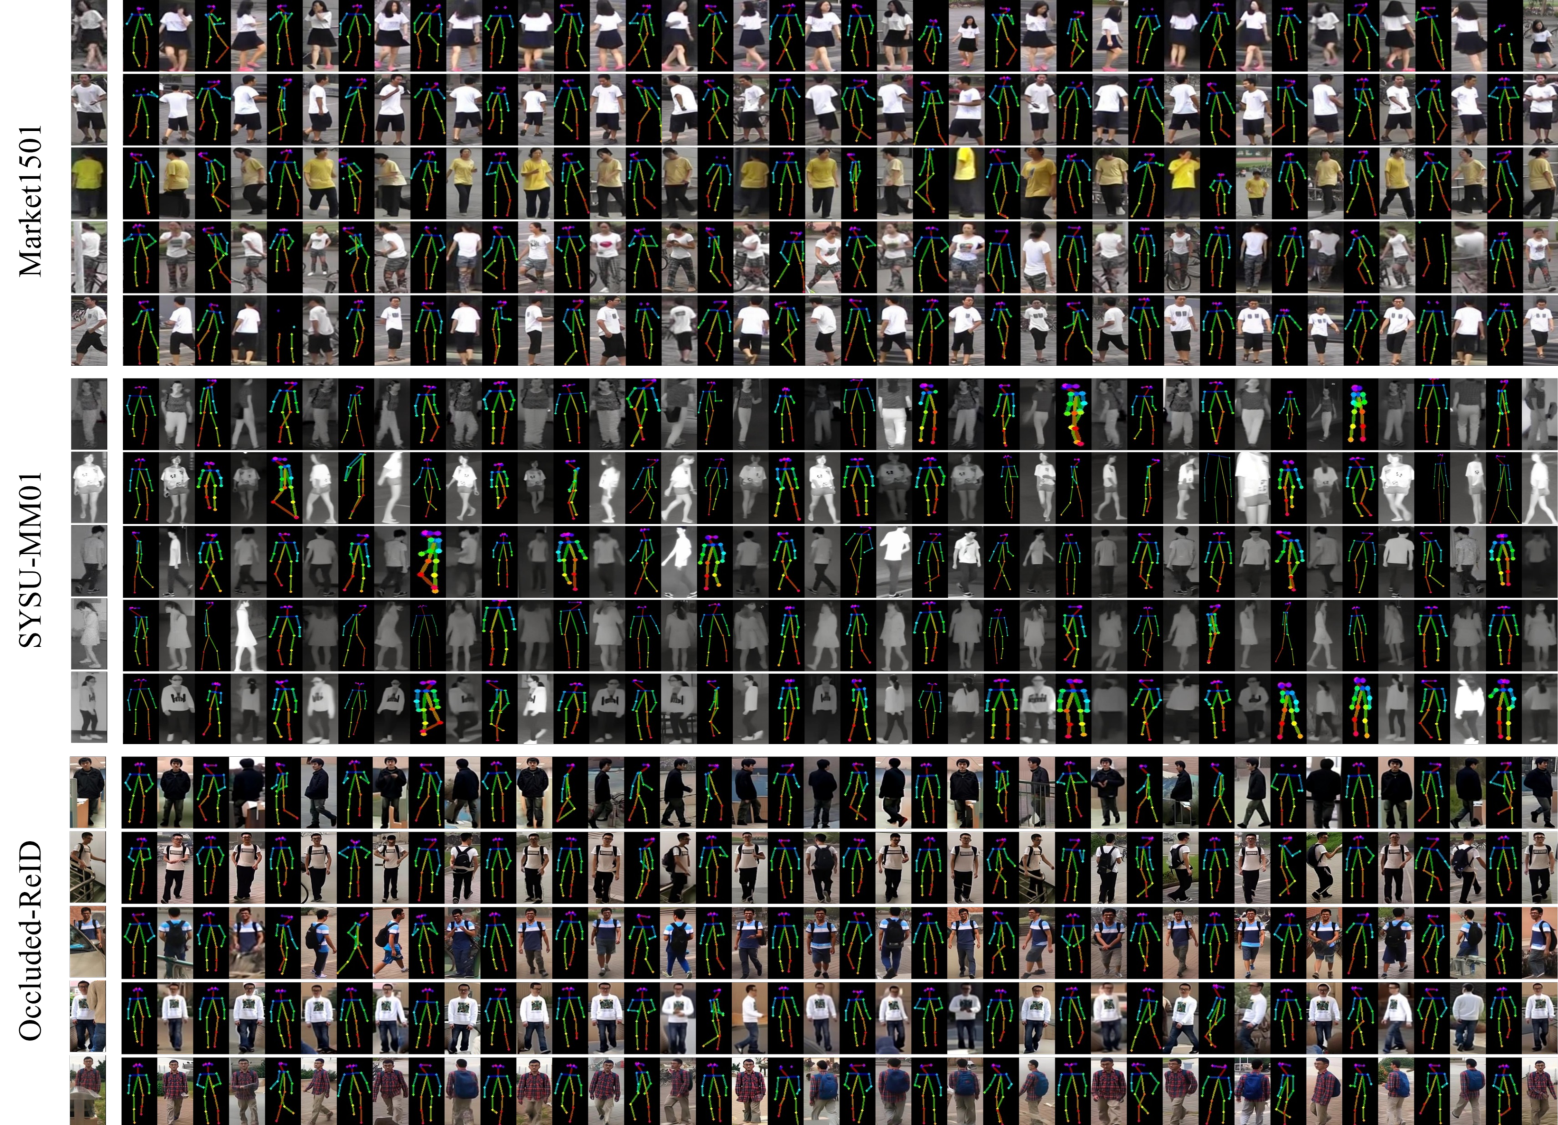
\includegraphics[width=\linewidth]{figs/pdf/random_sub_png.pdf}
\caption{Images generated with random poses. More randomly generated images can be found in Supplementary.}
\label{fig:randompose}
\end{figure*}
\\
\textbf{Effect of Feature Re-Distribute Module.}
We randomly selected 7 images from the Market1501 dataset, choosing 5 different poses for each image. We visualized the results both with and without Identity Feature Redistribute (IFR) Module. As shown in Fig.\ref{fig:IFR}, the impact of ID features on the generated outcomes is evident.
\\
\textbf{Effect of numbers of generated images.}
We randomly selected different numbers of images generated from the 8 representative poses to verify the effect of feature enhancement. As shown in Tab.\ref{tab:num}, the experimental results align with the theory mentioned in Section\ref{Feature Distribution}: the more features of the same ID that are aggregated, the more the adjustment noise extracted from individual images is reduced, enhancing the ID representation capability and resulting in improved matching performance.



\subsection{Visualizations}

\textbf{Different people with the same poses across datasets.}
We are working on Market1501, SYSU-MM01, and
Occluded-ReID datasets to visualize the 8 representative poses with only one model and results are shown in Fig.\ref{fig:intro}.
\\
\textbf{Random people with random poses.} To demonstrate the advancement of our model, as shown in Fig.\ref{fig:randompose}, we randomly chose samples from the whole dataset, and each sample randomly chose poses, including some problematic poses, fully demonstrating the diversity of model. \textbf{More examples on three datasets are visualized in }\textbf{Supplementary}.


% \subsection{Analysis on quality coefficient $\eta$ of Generation Model}

% Fig.\ref{fig:eta} illustrates the effect of adjusting the coefficient $\eta$ on the performance of the ReID model. To evaluate this impact, we gradually increased the value of $\eta$ and observed the changes in model performance on the mAP and Rank-1 metrics. 

% As the value of $\eta$ increases, the performance of the ReID model improves, reaching an optimal point. At $\eta = 2$, both mAP and Rank-1 achieve their maximum values of 88.02\% and 94.77\%, respectively. However, further increasing $\eta$ beyond this point leads to a slight decline in performance. It is easy to find that using generated images to centralize features is effective. However, considering the quality of the generated image, direct adding, although also effective, may not always achieve the best results. Therefore adjusting $\eta$ according to the generation quality of the model in this dataset can better centralize the features.
% \begin{figure}
% \centering
% 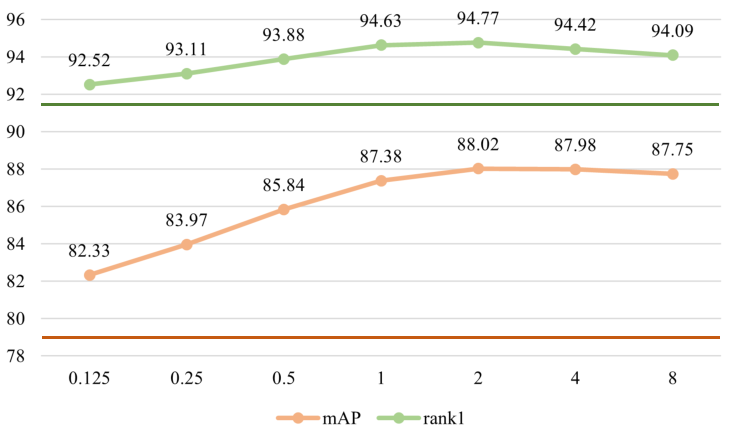
\includegraphics[width=0.9\linewidth]{figs/pdf/eta.pdf}
% \caption{Impact of the quality coefficient \( \eta \) with TransReID on Market1501. The dark color lines are the baseline.}
% \label{fig:eta}
% \end{figure}
\section{Conclusion}
\label{sec:conclusion}
In this work, we propose IDEA, a novel feature learning framework for multi-modal object ReID.
%
We first construct three text-enhanced multi-modal object ReID benchmarks using MLLMs, providing a structured caption generation pipeline.
%
With the generated text, the Inverted Multi-modal Feature Extractor (IMFE) leverages semantic guidance from inverted texts while reducing fusion conflicts.
%
Additionally, the Cooperative Deformable Aggregation (CDA) adaptively aggregates discriminative local features with global information.
%
Experiments on three public ReID benchmarks demonstrate the effectiveness of our method.
%
\\
{\small
\textbf{Acknowledgements.}
This work was supported in part by the National Natural Science Foundation of China (No. 62101092, 62476044, 62388101) and Open Project of Anhui Provincial Key Laboratory of Multimodal Cognitive Computation, Anhui University (No. MMC202102, MMC202407).} % 这里结束 \small 的作用范围
\vspace*{-4mm} 
{
    \small
    \bibliographystyle{ieeenat_fullname}
    \bibliography{cvpr25}
}
\clearpage
\appendix
\setcounter{page}{1}
\maketitlesupplementary

\section{Implementation Details}
We follow prior studies\cite{coop, cocoop, prograd, kgcoop, maple, tcp, mma} and adopt a 16-shot learning setting across all experiments, except for the few-shot learning tasks. The ViT-B/16\cite{vit} variant of the CLIP model serves as the visual backbone for all experimental setups. Hand-crafted text prompts from prior methods\cite{clip, coop, tip-adapter} are utilized and described in detail in \cref{datasets}. Optimization is performed using the AdamW optimizer with an initial learning rate of 0.001. All our models are trained with mix-precision for speeding up. For the larger ImageNet dataset, we employ a batch size of 32, while a batch size of 4 is used for all other datasets. Training on ImageNet for the base-to-novel generalization task spans 5 epochs, whereas training on the remaining datasets is conducted over 10 epochs. For cross-dataset evaluation and domain generalization tasks, we perform training for a single epoch on ImageNet. In the few-shot learning tasks, training is carried out for 5 epochs on ImageNet and 50 epochs for other datasets. The average accuracy is reported over three independent runs, with all experiments executed on a single NVIDIA RTX 4090 GPU.

Representation tokens are initialized from a zero-mean Gaussian distribution with a standard deviation of 0.02. We set $J = 6$, integrating the representation tokens beginning at the 6-th transformer layer. The dimension of the representation space, $d_r$, is set to 2048 for EuroSAT and 512 for all other datasets. Note that since the $d_r$ setting for EuroSAT differs from other datasets, in the $d_r$ ablation experiments we fix $d_r$ for EuroSAT to 2048 while adjusting $d_r$ on the other datasets. The number of representation tokens, $K$, is configured to 5. The parameter $\alpha$ is fixed at 0.7, and the details regarding the configuration of $\lambda$ are provided in \cref{ablation_lambda}.



\section{Dataset Details}
Details of 14 datasets are shown in \cref{datasets}.


\section{Computational Cost}
Table \ref{computational_cost} summarizes the learnable parameters, training time per image, total training duration, inference speed (measured in frames per second, FPS, with a batch size of 100), and the final HM metric for each approach. Our proposed model, MMRL, demonstrates a compelling balance of computational efficiency and performance. The key observations are as follows:
\begin{itemize}
    \item Models incorporating multimodal interaction mechanisms (e.g., MaPLe, MMA, and MMRL) generally involve a higher parameter count compared to models without such mechanisms.
    \item Both MMRL and the prior MMA approach exhibit significantly faster training speed, thereby reducing overall computational costs. While MaPLe and PromptSRC achieve higher inference speeds, their training durations are relatively longer. Notably, MMRL offers faster inference compared to MMA and MetaPrompt.
    \item To assess the performance of MMRL under constrained computational resources, we reduced the dimensionality of the representation space from 512 to 32. In this configuration, MMRL achieves a parameter count comparable to that of MMA, while still significantly outperforming the previous state-of-the-art model.
\end{itemize}



\begin{table}[h]
\centering
\renewcommand\arraystretch{1.25}
\caption{All methods were trained on a single NVIDIA RTX 4090 GPU using the ImageNet dataset. Each model was implemented with publicly available code and default configurations as described in their respective papers \cite{maple, promptsrc, provp, metaprompt, tcp, mma}. `V-L' denotes vision-language interaction, indicating that efficient fine-tuning incorporates interactions between visual and textual modalities before prediction. `V, L' signifies separate fine-tuning of each modality without inter-modal interaction before prediction, while `L' refers to fine-tuning limited to the textual modality alone. `Train time' is reported as both time per image and the total duration for training the full dataset(16-shots), while `FPS (100 BS)' indicates frames per second with a batch size of 100 during inference.}
\label{computational_cost}
\resizebox{0.475\textwidth}{!}{
    \begin{tabular}{@{}l|ccccc|c@{}}
    \toprule
    \multirow{2}{*}{Method} & \multirow{2}{*}{Modality} & Params & Train time & Train time & FPS & \multirow{2}{*}{HM} \\
               &     & (learnable) & (ms/image) & (minute/all) & (100 BS) &       \\ \midrule
    MaPLe      & V-L & 3.555M      & 39.5       & 26.4         & 1757.6   & 78.55 \\
    PromptSRC  & V,L & 0.046M      & 40.0       & 106.8        & 1764.2   & 79.97 \\
    ProVP      & V   & 0.147M      & 4.4        & 107.2        & 928.9    & 78.76 \\
    MetaPrompt & V,L & 0.031M      & 30.7       & 32.8         & 659.8    & 79.09 \\
    TCP        & L   & 0.332M      & 5.3        & 17.7         & 950.6    & 79.51 \\
    MMA        & V-L & 0.675M      & 2.2        & 1.5          & 688.5    & 79.87 \\ \midrule
    MMRL       & V-L & 4.992M      & 5.3        & 3.6          & 762.4    & 81.20 \\
    MMRL*      & V-L & 0.689M      & 5.3        & 3.6          & 767.8    & 80.84 \\ \bottomrule
    \end{tabular}
}
\end{table}


\section{Ablation Analysis on $\lambda$}
As shown in \cref{ablation_lambda}, increasing the value of $\lambda$ generally improves performance, with the optimal or near-optimal results typically observed when $\lambda$ is set between 4 and 6 across most datasets. Notably, as $\lambda$ continues to increase, its impact on model performance within the same dataset diminishes, indicating reduced sensitivity to variations in $\lambda$. This trend suggests that the model becomes more robust and less reliant on precise tuning of $\lambda$ at higher values.


\begin{table*}[h]
\centering
\caption{Summary of the 14 datasets.}
\label{datasets}
\renewcommand\arraystretch{1.2}
\resizebox{1.0\textwidth}{!}{
    \begin{tabular}{@{}l|llllll@{}}
    \toprule
    Dataset      & Classes & Train  & Val    & Test   & Description                         & Prompt                                \\ \midrule
    ImageNet     & 1000    & 1.28M  & $\sim$ & 50000  & Recognition of generic objects      & ``a photo of a [CLASS].”              \\
    Caltech101   & 100     & 4128   & 1649   & 2465   & Recognition of generic objects      & ``a photo of a [CLASS].”              \\
    OxfordPets      & 37    & 2944   & 736    & 3669   & Fine-grained classification of pets                    & ``a photo of a [CLASS], a type of pet.”      \\
    StanfordCars & 196     & 6509   & 1635   & 8041   & Fine-grained classification of cars & ``a photo of a [CLASS].”              \\
    Flowers102      & 102   & 4093   & 1633   & 2463   & Fine-grained classification of flowers                 & ``a photo of a [CLASS], a type of flower.”   \\
    Food101         & 101   & 50500  & 20200  & 30300  & Fine-grained classification of foods                   & ``a photo of [CLASS], a type of food.”       \\
    FGVCAircraft    & 100   & 3334   & 3333   & 3333   & Fine-grained classification of aircrafts               & ``a photo of a [CLASS], a type of aircraft.” \\
    SUN397       & 397     & 15880  & 3970   & 19850  & Scene classification                & ``a photo of a [CLASS].”              \\
    DTD          & 47      & 2820   & 1128   & 1692   & Texture classification              & ``[CLASS] texture.”                   \\
    EuroSAT         & 10    & 13500  & 5400   & 8100   & Land use \& cover classification with satellite images & ``a centered satellite photo of [CLASS].”    \\
    UCF101       & 101     & 7639   & 1898   & 3783   & Action recognition                  & ``a photo of a person doing [CLASS].” \\ \midrule
    ImageNetV2   & 1,000   & $\sim$ & $\sim$ & 10,000 & New test data for ImageNet          & ``a photo of a [CLASS].”              \\
    ImageNet-Sketch & 1,000 & $\sim$ & $\sim$ & 50,889 & Sketch-style images of ImageNet classes                & ``a photo of a [CLASS].”                     \\
    ImageNet-A      & 200   & $\sim$ & $\sim$ & 7,500  & Natural adversarial examples of 200 ImageNet classes   & ``a photo of a [CLASS].”                     \\
    ImageNet-R   & 200     & $\sim$ & $\sim$ & 30,000 & Renditions of 200 ImageNet classes  & ``a photo of a [CLASS].”              \\ \bottomrule
    \end{tabular}
    }
\end{table*}


\begin{table*}[h]
\centering
\caption{Ablation on $\lambda$ across 11 datasets, with results evaluated using the harmonic mean (HM) metric.}
\label{ablation_lambda}
\renewcommand\arraystretch{1.2}
\resizebox{1.0\textwidth}{!}{
    \begin{tabular}{@{}c|ccccccccccc@{}}
    \toprule
    $\alpha$ & ImageNet       & Caltech101     & OxfordPets & StanfordCars & Flowers102 & Food101 & FGVCAircraft   & SUN397         & DTD            & EuroSAT & UCF101 \\ \midrule
    0.0  & 74.01 & 95.97 & 96.35          & 76.00          & 84.42          & 90.10          & 38.52 & 79.67 & 68.21 & 82.65          & 81.63          \\
    0.01 & 74.07 & 96.12 & 96.39          & 75.95          & 84.82          & 90.23          & 37.87 & 79.85 & 67.73 & \textbf{87.21} & 82.11          \\
    0.1  & 74.23 & 96.25 & 96.49          & 76.32          & 84.81          & 90.53          & 38.66 & 80.23 & 69.79 & 83.21          & 82.91          \\
    0.2  & 74.38 & 96.40 & \textbf{96.74} & 76.67          & 85.31          & 90.61          & 39.27 & 80.25 & 70.58 & 82.68          & 82.70          \\
    0.5      & \textbf{74.45} & \textbf{96.68} & 96.54      & 77.09        & 85.74      & 90.86   & 40.37          & 80.61          & 72.67          & 82.87   & 83.05  \\
    3.0  & 74.09 & 96.59 & 96.51          & 77.72          & 86.65          & 90.98          & 40.48 & 81.10 & 73.54 & 77.95          & \textbf{83.89} \\
    4.0  & 74.04 & 96.62 & 96.55          & 77.73          & \textbf{86.78} & 90.98          & 40.66 & 81.14 & 73.75 & 77.27          & 83.45          \\
    5.0  & 73.93 & 96.62 & 96.60          & 77.86          & 86.42          & \textbf{91.03} & 40.42 & 81.07 & 73.69 & 78.05          & 83.84          \\
    6.0      & 73.83          & 96.61          & 96.66      & 78.05        & 86.48      & 91.00   & \textbf{41.15} & \textbf{81.20} & \textbf{73.82} & 75.23   & 83.68  \\
    7.0  & 73.78 & 96.62 & 96.58          & \textbf{78.06} & 86.53          & 90.95          & 40.88 & 81.10 & 73.65 & 75.85          & 83.55          \\
    10.0 & 73.68 & 96.64 & 96.56          & 77.86          & 86.46          & 91.00          & 41.01 & 80.93 & 73.68 & 77.61          & 83.38          \\ \bottomrule
    \end{tabular}
}
\end{table*}

\begin{table}[t]
\small
\centering
\caption{Ablation on different regularization strategies.}
\label{ablation_regularization}
\begin{tabular}{@{}c|ccc@{}}
\toprule
Regularization & Base           & Novel          & HM             \\ \midrule
\rowcolor[HTML]{EFEFEF} 
Cosine         & \textbf{85.68} & \textbf{77.16} & \textbf{81.20} \\
L1             & 85.46          & 76.03          & 80.47          \\
MSE             & 85.13          & 74.62          & 79.53          \\ \bottomrule
\end{tabular}
\end{table}

\section{Ablation Analysis on Regularization Strategies}
We investigate the impact of various regularization strategies aimed at maximizing the similarity between class token features and frozen CLIP features to retain pre-trained knowledge. The results, summarized in \cref{ablation_regularization}, indicate that cosine regularization achieves the best performance. In contrast, both L1 and MSE losses lead to performance degradation, with MSE causing a significant decline. This result can be attributed to the more relaxed and flexible constraints of cosine regularization, enabling the class token to preserve generalizability while effectively capturing task-specific knowledge.






\section{Few-Shot Learning}
\cref{few_shot1,few_shot2} provide detailed comparisons of MMRL and prior state-of-the-art methods on few-shot learning across 11 datasets. MMRL achieves the highest average performance across all shots. Note that the MMA results are reproduced from the open-source code, as the original paper does not report results for this experiment.







\begin{table*}[t]
\small
\centering
\caption{Comparison of MMRL with previous state-of-the-art methods on few-shot learning across 11 datasets.}
\label{few_shot1}
\setlength{\tabcolsep}{15pt}{
\resizebox{0.9\textwidth}{!}{
    \begin{tabular}{@{}ll|ccccc}
    \toprule
    \textbf{Dataset} &
      \textbf{Method} &
      \textbf{1 shot} &
      \textbf{2 shots} &
      \textbf{4 shots} &
      \textbf{8 shots} &
      \textbf{16 shots} \\ \midrule
     &
      Linear probe CLIP &
      45.83 &
      57.98 &
      68.01 &
      74.47 &
      78.79 \\
     &
      CoOp &
      67.56 &
      70.65 &
      74.02 &
      76.98 &
      79.89 \\
     &
      CoCoOp &
      66.79 &
      67.65 &
      71.21 &
      72.96 &
      74.90 \\
     &
      MaPLe &
      69.27 &
      72.58 &
      75.37 &
      78.89 &
      81.79 \\
     &
      PromptSRC &
      72.32 &
      75.29 &
      78.35 &
      80.69 &
      82.87 \\
     &
      MMA &
      69.28 &
      72.08 &
      76.38 &
      79.57 &
      82.76 \\
    \multirow{-7}{*}{Average} &
      \cellcolor[HTML]{E8E8E8}$\text{MMRL}_{\text{ (Ours)}}$ &
      \cellcolor[HTML]{E8E8E8}\textbf{72.67} &
      \cellcolor[HTML]{E8E8E8}\textbf{75.90} &
      \cellcolor[HTML]{E8E8E8}\textbf{79.20} &
      \cellcolor[HTML]{E8E8E8}\textbf{81.47} &
      \cellcolor[HTML]{E8E8E8}\textbf{84.34} \\ \midrule
     &
      Linear probe CLIP &
      32.13 &
      44.88 &
      54.85 &
      62.23 &
      67.31 \\
     &
      CoOp &
      66.33 &
      67.07 &
      68.73 &
      70.63 &
      71.87 \\
     &
      CoCoOp &
      69.43 &
      69.78 &
      70.39 &
      70.63 &
      70.83 \\
     &
      MaPLe &
      62.67 &
      65.10 &
      67.70 &
      70.30 &
      72.33 \\
     &
      PromptSRC &
      68.13 &
      69.77 &
      71.07 &
      \textbf{72.33} &
      73.17 \\
     &
      MMA &
      \textbf{69.17} &
      \textbf{70.37} &
      71.00 &
      71.77 &
      73.13 \\
    \multirow{-7}{*}{ImageNet} &
      \cellcolor[HTML]{E8E8E8}$\text{MMRL}_{\text{ (Ours)}}$ &
      \cellcolor[HTML]{E8E8E8}69.00 &
      \cellcolor[HTML]{E8E8E8}70.30 &
      \cellcolor[HTML]{E8E8E8}\textbf{71.40} &
      \cellcolor[HTML]{E8E8E8}\textbf{72.33} &
      \cellcolor[HTML]{E8E8E8}\textbf{73.40} \\ \midrule
     &
      Linear probe CLIP &
      79.88 &
      89.01 &
      92.05 &
      93.41 &
      95.43 \\
     &
      CoOp &
      92.60 &
      93.07 &
      94.40 &
      94.37 &
      95.57 \\
     &
      CoCoOp &
      93.83 &
      94.82 &
      94.98 &
      95.04 &
      95.16 \\
     &
      MaPLe &
      92.57 &
      93.97 &
      94.43 &
      95.20 &
      96.00 \\
     &
      PromptSRC &
      93.67 &
      94.53 &
      95.27 &
      95.67 &
      96.07 \\
     &
      MMA &
      92.90 &
      94.00 &
      94.33 &
      95.37 &
      96.33 \\
    \multirow{-7}{*}{Caltech101} &
      \cellcolor[HTML]{E8E8E8}$\text{MMRL}_{\text{ (Ours)}}$ &
      \cellcolor[HTML]{E8E8E8}\textbf{94.17} &
      \cellcolor[HTML]{E8E8E8}\textbf{94.83} &
      \cellcolor[HTML]{E8E8E8}\textbf{96.03} &
      \cellcolor[HTML]{E8E8E8}\textbf{96.27} &
      \cellcolor[HTML]{E8E8E8}\textbf{97.13} \\ \midrule
     &
      Linear probe CLIP &
      44.06 &
      58.37 &
      71.17 &
      78.36 &
      85.34 \\
     &
      CoOp &
      90.37 &
      89.80 &
      92.57 &
      91.27 &
      91.87 \\
     &
      CoCoOp &
      91.27 &
      \textbf{92.64} &
      92.81 &
      93.45 &
      93.34 \\
     &
      MaPLe &
      89.10 &
      90.87 &
      91.90 &
      92.57 &
      92.83 \\
     &
      PromptSRC &
      \textbf{92.00} &
      92.50 &
      \textbf{93.43} &
      \textbf{93.50} &
      93.67 \\
     &
      MMA &
      91.23 &
      91.97 &
      92.23 &
      92.77 &
      93.23 \\
    \multirow{-7}{*}{OxfordPets} &
      \cellcolor[HTML]{E8E8E8}$\text{MMRL}_{\text{ (Ours)}}$ &
      \cellcolor[HTML]{E8E8E8}90.87 &
      \cellcolor[HTML]{E8E8E8}91.57 &
      \cellcolor[HTML]{E8E8E8}92.57 &
      \cellcolor[HTML]{E8E8E8}93.03 &
      \cellcolor[HTML]{E8E8E8}\textbf{93.83} \\ \midrule
     &
      Linear probe CLIP &
      35.66 &
      50.28 &
      63.38 &
      73.67 &
      80.44 \\
     &
      CoOp &
      67.43 &
      70.50 &
      74.47 &
      79.30 &
      83.07 \\
     &
      CoCoOp &
      67.22 &
      68.37 &
      69.39 &
      70.44 &
      71.57 \\
     &
      MaPLe &
      66.60 &
      71.60 &
      75.30 &
      79.47 &
      83.57 \\
     &
      PromptSRC &
      \textbf{69.40} &
      \textbf{73.40} &
      77.13 &
      80.97 &
      83.83 \\
     &
      MMA &
      67.87 &
      71.77 &
      76.50 &
      81.40 &
      85.70 \\
    \multirow{-7}{*}{StanfordCars} &
      \cellcolor[HTML]{E8E8E8}$\text{MMRL}_{\text{ (Ours)}}$ &
      \cellcolor[HTML]{E8E8E8}68.70 &
      \cellcolor[HTML]{E8E8E8}72.93 &
      \cellcolor[HTML]{E8E8E8}\textbf{78.17} &
      \cellcolor[HTML]{E8E8E8}\textbf{82.57} &
      \cellcolor[HTML]{E8E8E8}\textbf{86.43} \\ \midrule
     &
      Linear probe CLIP &
      69.74 &
      85.07 &
      92.02 &
      96.10 &
      97.37 \\
     &
      CoOp &
      77.53 &
      87.33 &
      92.17 &
      94.97 &
      97.07 \\
     &
      CoCoOp &
      72.08 &
      75.79 &
      78.40 &
      84.30 &
      87.84 \\
     &
      MaPLe &
      83.30 &
      88.93 &
      92.67 &
      95.80 &
      97.00 \\
     &
      PromptSRC &
      85.93 &
      91.17 &
      93.87 &
      96.27 &
      97.60 \\
     &
      MMA &
      83.60 &
      90.30 &
      93.00 &
      95.97 &
      97.97 \\
    \multirow{-7}{*}{Flowers102} &
      \cellcolor[HTML]{E8E8E8}$\text{MMRL}_{\text{ (Ours)}}$ &
      \cellcolor[HTML]{E8E8E8}\textbf{85.97} &
      \cellcolor[HTML]{E8E8E8}\textbf{91.20} &
      \cellcolor[HTML]{E8E8E8}\textbf{94.60} &
      \cellcolor[HTML]{E8E8E8}\textbf{96.60} &
      \cellcolor[HTML]{E8E8E8}\textbf{98.40} \\ \bottomrule
    \end{tabular}
    }
    }
\end{table*}


\begin{table*}[t]
\small
\centering
\caption{Comparison of MMRL with previous state-of-the-art methods on few-shot learning across 11 datasets.}
\label{few_shot2}
\setlength{\tabcolsep}{15pt}{
\resizebox{0.9\textwidth}{!}{
    \begin{tabular}{@{}ll|ccccc}
    \toprule
    \textbf{Dataset} &
      \textbf{Method} &
      \textbf{1 shot} &
      \textbf{2 shots} &
      \textbf{4 shots} &
      \textbf{8 shots} &
      \textbf{16 shots} \\ \midrule
     &
      Linear probe CLIP &
      43.96 &
      61.51 &
      73.19 &
      79.79 &
      82.90 \\
     &
      CoOp &
      84.33 &
      84.40 &
      84.47 &
      82.67 &
      84.20 \\
     &
      CoCoOp &
      \textbf{85.65} &
      \textbf{86.22} &
      \textbf{86.88} &
      \textbf{86.97} &
      87.25 \\
     &
      MaPLe &
      80.50 &
      81.47 &
      81.77 &
      83.60 &
      85.33 \\
     &
      PromptSRC &
      84.87 &
      85.70 &
      86.17 &
      86.90 &
      \textbf{87.50} \\
     &
      MMA &
      83.03 &
      82.50 &
      82.13 &
      83.00 &
      84.57 \\
    \multirow{-7}{*}{Food101} &
      \cellcolor[HTML]{E8E8E8}$\text{MMRL}_{\text{ (Ours)}}$ &
      \cellcolor[HTML]{E8E8E8}84.87 &
      \cellcolor[HTML]{E8E8E8}85.53 &
      \cellcolor[HTML]{E8E8E8}85.77 &
      \cellcolor[HTML]{E8E8E8}86.33 &
      \cellcolor[HTML]{E8E8E8}87.03 \\ \midrule
     &
      Linear probe CLIP &
      19.61 &
      26.41 &
      32.33 &
      39.35 &
      45.36 \\
     &
      CoOp &
      21.37 &
      26.20 &
      30.83 &
      39.00 &
      43.40 \\
     &
      CoCoOp &
      12.68 &
      15.06 &
      24.79 &
      26.61 &
      31.21 \\
     &
      MaPLe &
      26.73 &
      30.90 &
      34.87 &
      42.00 &
      48.40 \\
     &
      PromptSRC &
      27.67 &
      31.70 &
      37.47 &
      43.27 &
      50.83 \\
     &
      MMA &
      \textbf{28.73} &
      31.90 &
      37.57 &
      44.83 &
      52.70 \\
    \multirow{-7}{*}{FGVCAircraft} &
      \cellcolor[HTML]{E8E8E8}$\text{MMRL}_{\text{ (Ours)}}$ &
      \cellcolor[HTML]{E8E8E8}28.53 &
      \cellcolor[HTML]{E8E8E8}\textbf{34.23} &
      \cellcolor[HTML]{E8E8E8}\textbf{40.47} &
      \cellcolor[HTML]{E8E8E8}\textbf{48.07} &
      \cellcolor[HTML]{E8E8E8}\textbf{57.60} \\ \midrule
     &
      Linear probe CLIP &
      41.58 &
      53.70 &
      63.00 &
      69.08 &
      73.28 \\
     &
      CoOp &
      66.77 &
      66.53 &
      69.97 &
      71.53 &
      74.67 \\
     &
      CoCoOp &
      68.33 &
      69.03 &
      70.21 &
      70.84 &
      72.15 \\
     &
      MaPLe &
      64.77 &
      67.10 &
      70.67 &
      73.23 &
      75.53 \\
     &
      PromptSRC &
      \textbf{69.67} &
      \textbf{71.60} &
      \textbf{74.00} &
      75.73 &
      77.23 \\
     &
      MMA &
      64.00 &
      67.17 &
      69.97 &
      72.30 &
      74.63 \\
    \multirow{-7}{*}{SUN397} &
      \cellcolor[HTML]{E8E8E8}$\text{MMRL}_{\text{ (Ours)}}$ &
      \cellcolor[HTML]{E8E8E8}68.90 &
      \cellcolor[HTML]{E8E8E8}71.53 &
      \cellcolor[HTML]{E8E8E8}73.93 &
      \cellcolor[HTML]{E8E8E8}\textbf{76.00} &
      \cellcolor[HTML]{E8E8E8}\textbf{77.70} \\ \midrule
     &
      Linear probe CLIP &
      34.59 &
      40.76 &
      55.71 &
      63.46 &
      69.96 \\
     &
      CoOp &
      50.23 &
      53.60 &
      58.70 &
      64.77 &
      69.87 \\
     &
      CoCoOp &
      48.54 &
      52.17 &
      55.04 &
      58.89 &
      63.04 \\
     &
      MaPLe &
      52.13 &
      55.50 &
      61.00 &
      66.50 &
      71.33 \\
     &
      PromptSRC &
      56.23 &
      59.97 &
      65.53 &
      69.87 &
      72.73 \\
     &
      MMA &
      52.27 &
      56.90 &
      63.93 &
      67.97 &
      73.47 \\
    \multirow{-7}{*}{DTD} &
      \cellcolor[HTML]{E8E8E8}$\text{MMRL}_{\text{ (Ours)}}$ &
      \cellcolor[HTML]{E8E8E8}\textbf{56.37} &
      \cellcolor[HTML]{E8E8E8}\textbf{61.37} &
      \cellcolor[HTML]{E8E8E8}\textbf{67.87} &
      \cellcolor[HTML]{E8E8E8}\textbf{71.60} &
      \cellcolor[HTML]{E8E8E8}\textbf{75.30} \\ \midrule
     &
      Linear probe CLIP &
      49.23 &
      61.98 &
      77.09 &
      84.43 &
      87.21 \\
     &
      CoOp &
      54.93 &
      65.17 &
      70.80 &
      78.07 &
      84.93 \\
     &
      CoCoOp &
      55.33 &
      46.74 &
      65.56 &
      68.21 &
      73.32 \\
     &
      MaPLe &
      71.80 &
      78.30 &
      84.50 &
      87.73 &
      92.33 \\
     &
      PromptSRC &
      73.13 &
      79.37 &
      86.30 &
      \textbf{88.80} &
      92.43 \\
     &
      MMA &
      55.07 &
      59.80 &
      79.40 &
      86.47 &
      92.37 \\
    \multirow{-7}{*}{EuroSAT} &
      \cellcolor[HTML]{E8E8E8}$\text{MMRL}_{\text{ (Ours)}}$ &
      \cellcolor[HTML]{E8E8E8}\textbf{76.00} &
      \cellcolor[HTML]{E8E8E8}\textbf{82.87} &
      \cellcolor[HTML]{E8E8E8}\textbf{87.67} &
      \cellcolor[HTML]{E8E8E8}88.73 &
      \cellcolor[HTML]{E8E8E8}\textbf{93.37} \\ \midrule
     &
      Linear probe CLIP &
      53.66 &
      65.78 &
      73.28 &
      79.34 &
      82.11 \\
     &
      CoOp &
      71.23 &
      73.43 &
      77.10 &
      80.20 &
      82.23 \\
     &
      CoCoOp &
      70.30 &
      73.51 &
      74.82 &
      77.14 &
      78.14 \\
     &
      MaPLe &
      71.83 &
      74.60 &
      78.47 &
      81.37 &
      85.03 \\
     &
      PromptSRC &
      74.80 &
      \textbf{78.50} &
      81.57 &
      84.30 &
      86.47 \\
     &
      MMA &
      74.17 &
      76.17 &
      80.10 &
      83.43 &
      86.30 \\
    \multirow{-7}{*}{UCF101} &
      \cellcolor[HTML]{E8E8E8}$\text{MMRL}_{\text{ (Ours)}}$ &
      \cellcolor[HTML]{E8E8E8}\textbf{75.97} &
      \cellcolor[HTML]{E8E8E8}\textbf{78.50} &
      \cellcolor[HTML]{E8E8E8}\textbf{82.67} &
      \cellcolor[HTML]{E8E8E8}\textbf{84.67} &
      \cellcolor[HTML]{E8E8E8}\textbf{87.60} \\ \bottomrule
    \end{tabular}
    }
    }
\end{table*}




\end{document}
